\documentclass{beamer}

% xcolor and define colors -------------------------
\usepackage{xcolor}

% https://www.viget.com/articles/color-contrast/
\definecolor{purple}{HTML}{5601A4}
\definecolor{navy}{HTML}{0D3D56}
\definecolor{ruby}{HTML}{9a2515}
\definecolor{alice}{HTML}{107895}
\definecolor{daisy}{HTML}{EBC944}
\definecolor{coral}{HTML}{F26D21}
\definecolor{kelly}{HTML}{829356}
\definecolor{cranberry}{HTML}{E64173}
\definecolor{jet}{HTML}{131516}
\definecolor{asher}{HTML}{555F61}
\definecolor{slate}{HTML}{314F4F}

% Mixtape Sessions
\definecolor{picton-blue}{HTML}{00b7ff}
\definecolor{violet-red}{HTML}{ff3881}
\definecolor{sun}{HTML}{ffaf18}
\definecolor{electric-violet}{HTML}{871EFF}

% Main theme colors
\definecolor{accent}{HTML}{00b7ff}
\definecolor{accent2}{HTML}{871EFF}
\definecolor{gray100}{HTML}{f3f4f6}
\definecolor{gray800}{HTML}{1F292D}


% Beamer Options -------------------------------------

% Background
\setbeamercolor{background canvas}{bg = white}

% Change text margins
\setbeamersize{text margin left = 15pt, text margin right = 15pt} 

% \alert
\setbeamercolor{alerted text}{fg = accent2}

% Frame title
\setbeamercolor{frametitle}{bg = white, fg = jet}
\setbeamercolor{framesubtitle}{bg = white, fg = accent}
\setbeamerfont{framesubtitle}{size = \small, shape = \itshape}

% Block
\setbeamercolor{block title}{fg = white, bg = accent2}
\setbeamercolor{block body}{fg = gray800, bg = gray100}

% Title page
\setbeamercolor{title}{fg = gray800}
\setbeamercolor{subtitle}{fg = accent}

%% Custom \maketitle and \titlepage
\setbeamertemplate{title page}
{
    %\begin{centering}
        \vspace{20mm}
        {\Large \usebeamerfont{title}\usebeamercolor[fg]{title}\inserttitle}\\
        {\large \itshape \usebeamerfont{subtitle}\usebeamercolor[fg]{subtitle}\insertsubtitle}\\ \vspace{10mm}
        {\insertauthor}\\
        {\color{asher}\small{\insertdate}}\\
    %\end{centering}
}

% Table of Contents
\setbeamercolor{section in toc}{fg = accent!70!jet}
\setbeamercolor{subsection in toc}{fg = jet}

% Button 
\setbeamercolor{button}{bg = accent}

% Remove navigation symbols
\setbeamertemplate{navigation symbols}{}

% Table and Figure captions
\setbeamercolor{caption}{fg=jet!70!white}
\setbeamercolor{caption name}{fg=jet}
\setbeamerfont{caption name}{shape = \itshape}

% Bullet points

%% Fix left-margins
\settowidth{\leftmargini}{\usebeamertemplate{itemize item}}
\addtolength{\leftmargini}{\labelsep}

%% enumerate item color
\setbeamercolor{enumerate item}{fg = accent}
\setbeamerfont{enumerate item}{size = \small}
\setbeamertemplate{enumerate item}{\insertenumlabel.}

%% itemize
\setbeamercolor{itemize item}{fg = accent!70!white}
\setbeamerfont{itemize item}{size = \small}
\setbeamertemplate{itemize item}[circle]

%% right arrow for subitems
\setbeamercolor{itemize subitem}{fg = accent!60!white}
\setbeamerfont{itemize subitem}{size = \small}
\setbeamertemplate{itemize subitem}{$\rightarrow$}

\setbeamertemplate{itemize subsubitem}[square]
\setbeamercolor{itemize subsubitem}{fg = jet}
\setbeamerfont{itemize subsubitem}{size = \small}







% Links ----------------------------------------------

\usepackage{hyperref}
\hypersetup{
  colorlinks = true,
  linkcolor = accent2,
  filecolor = accent2,
  urlcolor = accent2,
  citecolor = accent2,
}


% Line spacing --------------------------------------
\usepackage{setspace}
\setstretch{1.2}


% \begin{columns} -----------------------------------
\usepackage{multicol}


% Fonts ---------------------------------------------
% Beamer Option to use custom fonts
\usefonttheme{professionalfonts}

% \usepackage[utopia, smallerops, varg]{newtxmath}
% \usepackage{utopia}
\usepackage[sfdefault,light]{roboto}

% Small adjustments to text kerning
\usepackage{microtype}



% Remove annoying over-full box warnings -----------
\vfuzz2pt 
\hfuzz2pt


% Table of Contents with Sections
\setbeamerfont{myTOC}{series=\bfseries, size=\Large}
\AtBeginSection[]{
        \frame{
            \frametitle{Roadmap}
            \tableofcontents[current]   
        }
    }


% Tables -------------------------------------------
% Tables too big
% \begin{adjustbox}{width = 1.2\textwidth, center}
\usepackage{adjustbox}
\usepackage{array}
\usepackage{threeparttable, booktabs, adjustbox}
    
% Fix \input with tables
% \input fails when \\ is at end of external .tex file
\makeatletter
\let\input\@@input
\makeatother

% Tables too narrow
% \begin{tabularx}{\linewidth}{cols}
% col-types: X - center, L - left, R -right
% Relative scale: >{\hsize=.8\hsize}X/L/R
\usepackage{tabularx}
\newcolumntype{L}{>{\raggedright\arraybackslash}X}
\newcolumntype{R}{>{\raggedleft\arraybackslash}X}
\newcolumntype{C}{>{\centering\arraybackslash}X}

% Figures

% \imageframe{img_name} -----------------------------
% from https://github.com/mattjetwell/cousteau
\newcommand{\imageframe}[1]{%
    \begin{frame}[plain]
        \begin{tikzpicture}[remember picture, overlay]
            \node[at = (current page.center), xshift = 0cm] (cover) {%
                \includegraphics[keepaspectratio, width=\paperwidth, height=\paperheight]{#1}
            };
        \end{tikzpicture}
    \end{frame}%
}

% subfigures
\usepackage{subfigure}


% Highlight slide -----------------------------------
% \begin{transitionframe} Text \end{transitionframe}
% from paulgp's beamer tips
\newenvironment{transitionframe}{
    \setbeamercolor{background canvas}{bg=accent!40!black}
    \begin{frame}\color{accent!10!white}\LARGE\centering
}{
    \end{frame}
}


% Table Highlighting --------------------------------
% Create top-left and bottom-right markets in tabular cells with a unique matching id and these commands will outline those cells
\usepackage[beamer,customcolors]{hf-tikz}
\usetikzlibrary{calc}
\usetikzlibrary{fit,shapes.misc}

% To set the hypothesis highlighting boxes red.
\newcommand\marktopleft[1]{%
    \tikz[overlay,remember picture] 
        \node (marker-#1-a) at (0,1.5ex) {};%
}
\newcommand\markbottomright[1]{%
    \tikz[overlay,remember picture] 
        \node (marker-#1-b) at (0,0) {};%
    \tikz[accent!80!jet, ultra thick, overlay, remember picture, inner sep=4pt]
        \node[draw, rectangle, fit=(marker-#1-a.center) (marker-#1-b.center)] {};%
}

\usepackage{breqn} % Breaks lines

\usepackage{amsmath}
\usepackage{mathtools}

\usepackage{pdfpages} % \includepdf

\usepackage{listings} % R code
\usepackage{verbatim} % verbatim

% Video stuff
\usepackage{media9}

% packages for bibs and cites
\usepackage{natbib}
\usepackage{har2nat}
\newcommand{\possessivecite}[1]{\citeauthor{#1}'s \citeyearpar{#1}}
\usepackage{breakcites}
\usepackage{alltt}

% tikz
\usepackage{tikz}
\usepackage{pgfplots}
\usetikzlibrary{calc, positioning, decorations.pathreplacing, arrows.meta, intersections}
\pgfdeclarelayer{bg}
\pgfdeclarelayer{back}
\pgfdeclarelayer{fg}
\pgfsetlayers{bg,main,fg,back}
\usetikzlibrary{shapes,arrows}

% Setup math operators
\DeclareMathOperator{\E}{E} \DeclareMathOperator{\tr}{tr} \DeclareMathOperator{\se}{se} \DeclareMathOperator{\I}{I} \DeclareMathOperator{\sign}{sign} \DeclareMathOperator{\supp}{supp} \DeclareMathOperator{\plim}{plim}
\DeclareMathOperator*{\dlim}{\mathnormal{d}\mkern2mu-lim}
\newcommand\independent{\protect\mathpalette{\protect\independenT}{\perp}}
   \def\independenT#1#2{\mathrel{\rlap{$#1#2$}\mkern2mu{#1#2}}}
\newcommand*\colvec[1]{\begin{pmatrix}#1\end{pmatrix}}

\newcommand{\myurlshort}[2]{\href{#1}{\textcolor{gray}{\textsf{#2}}}}


\begin{document}

\imageframe{./lecture_includes/mixtape_ci_cover.png}


% ---- Content ----

\section{Adjusting for Known and quantified Confounders}

\subsection{Backdoor criterion and model}

\begin{frame}{Controlling for variables}

\begin{itemize}
\item One of the first things you learn in a methods course is multivariate regression ``controlling for $X$''
\item What is this? Why do we do this?  What should $X$ be? What causal parameter does it help identify?
\item This section is traditionally taught under a variety of headings -- unconfoundedness, selection on observables, or by name (e.g., matching, subclassification)
\item For today I will call it ``adjusting for known and quantified confounders'' to emphasize the prerequisite knowledge
\end{itemize}

\end{frame}

\begin{frame}{Which covariates?}

\begin{itemize}

\item Traditionally, we learn about ``controlling for variables'' using regressions like $$Y_i = \alpha + \delta D_i + \beta X_i + \varepsilon_i$$
\item Today we will learn more about this method, as well as seek to understand situations where other methods may perform better
\item But before we do, we need to have a guide as to which variables to include and which ones not to
\item There'll be formal justifications, and there will be ad hoc ones

\end{itemize}

\end{frame}

\begin{frame}{Backdoor criterion}

\begin{itemize}

\item Recall that the value of causal graphs is that if you can make statements about the causal pathways into treatment and outcome, then certain model-based approaches emerge
\item One such approach is the backdoor criterion which states that if you can condition on $X$ such that all backdoor paths close, then you can identify some aggregate causal parameter
\item But this requires a model, and I don't mean a theoretical model that you might learn as some abstract theory about education
\item It's a model of treatment assignment, which is local in nature

\end{itemize}

\end{frame}

\begin{frame}{Simple DAG}

\begin{figure}
\begin{center}
\caption{A simple DAG illustrating selection on observables.}
\begin{tikzpicture}[node distance=2cm]
% nodes %
\node[text centered] (d) {$D$};
\node[below left of = d, text centered] (c) {$C$};
\node[above left of = d, text centered] (w) {$W$};
\node[right of = d, text centered] (y) {$Y$};
% edges %
\draw[->, line width= 1] (d) -- (y);
\draw[->, line width= 1] (c) -- (d);
\draw[->, line width= 1] (w) -- (d);
\draw[->, line width= 1] (c) -- (y);
\draw[->, line width= 1] (w) -- (y);
\end{tikzpicture}
\label{fig:backdoor_dag}
\end{center}
\end{figure}

\bigskip

Write down all paths, both direct from $D$ to $Y$ and indirect or ``backdoor paths'' 

\end{frame}

\begin{frame}{Simple DAG}

\begin{figure}
\begin{center}
\caption{A simple DAG illustrating selection on observables.}
\begin{tikzpicture}[node distance=2cm]
% nodes %
\node[text centered] (d) {$D$};
\node[below left of = d, text centered] (c) {$C$};
\node[above left of = d, text centered] (w) {$W$};
\node[right of = d, text centered] (y) {$Y$};
% edges %
\draw[->, line width= 1] (d) -- (y);
\draw[->, line width= 1] (c) -- (d);
\draw[->, line width= 1] (w) -- (d);
\draw[->, line width= 1] (c) -- (y);
\draw[->, line width= 1] (w) -- (y);
\end{tikzpicture}
\label{fig:backdoor_dag1}
\end{center}
\end{figure}

\bigskip

\begin{enumerate}
\item[1. ] $D\rightarrow Y$, the direct edge representing a causal effect with associated causal parameter like the ATE, ATT, etc. 
\end{enumerate}
\end{frame}



\begin{frame}{Simple DAG}

\begin{figure}
\begin{center}
\caption{The same simple DAG illustrating selection on observables only with the direct edge from $D$ to $Y$ deleted and backdoor $W$ blocked.}
\begin{tikzpicture}[node distance=2cm]
% nodes %
\node[text centered] (d) {$D$};
\node[below left of = d, text centered] (c) {$C$};
\node[above left of = d, text centered] (w) {$\mybox{W}$};
\node[right of = d, text centered] (y) {$Y$};
% edges %
\draw[->, line width= 1] (d) -- (y);
\draw[->, line width= 1] (c) -- (d);
\draw[->, line width= 1] (c) -- (y);
\end{tikzpicture}
\label{fig:backdoor_dag2}
\end{center}
\end{figure}

\bigskip

\begin{enumerate}
\item[2. ] $D\leftarrow \mybox{W} \rightarrow Y$ is a backdoor from $D$ to $Y$ through $W$. \textcolor{purple}{Block it}
\end{enumerate}
\end{frame}



\begin{frame}{Remaining variation after blocking}

\begin{figure}
\begin{center}
\caption{Visualization of Backdoor Criterion}
\begin{tikzpicture}[node distance=2cm]
% nodes %
\node[text centered] (d) {$D$};
\node[below left of = d, text centered] (c) {$\mybox{C}$};
\node[above left of = d, text centered] (w) {$\mybox{W}$};
\node[right of = d, text centered] (y) {$Y$};
% edges %
\draw[->, line width= 1] (d) -- (y);
\end{tikzpicture}
\label{fig:backdoor_dag}
\end{center}
\end{figure}

\bigskip

\begin{enumerate}
\item[2. ] $D\leftarrow \mybox{W} \rightarrow Y$ is a backdoor from $D$ to $Y$ through $W$. \textcolor{purple}{Block it}
\item[3. ] $D\leftarrow \mybox{C} \rightarrow Y$ is a backdoor from $D$ to $Y$ through $C$. \textcolor{purple}{Block it}
\end{enumerate}
\end{frame}


\subsection{Confounders, Covariates and Colliders}

\begin{frame}{Definition of Known and Quantified Confounders}
	
	
	\begin{block}{Definition of a Known and Quantified Confounder}
	Variable $C$ is a \emph{known} and \emph{quantified} \emph{confounders} if the researcher believes it causes units to select into treatment ($C \rightarrow D$) and also independently determine outcome $Y$, or $C \rightarrow Y$. Confounders are always known, which requires prior knowledge. And to be quantified, they must be correctly measured in your dataset.
	\end{block}
	
	
\end{frame}

\begin{frame}{Known and Quantified Confounder}

	\begin{itemize}
	\item Confounders may or may not be observed, but they must be known if they are confounders as confounders create backdoor paths from $D$ to $Y$
	\item Visually, solid lines means they are ``quantified'' (i.e., in the data), whereas dashed lines mean they are either not defined correctly or not in the dataset (``unobserved'')
	\item Backdoor criterion is appropriate only for known and quantified confounders -- if either known or quantified is missing, this material today is not to be used
	\end{itemize}

\end{frame}

\begin{frame}{DAG tells us what we need to condition on}

\begin{itemize}

\item If we ``block'' on $C$ and $W$, then the \emph{only} explanation of why $D$ and $Y$ are then correlated is causal
\item Depending on the model we estimate, and explicit assumptions made about potential outcomes, then we are able to identify an aggregate causal parameter
\item We call $C$ and $W$ the ``known and quantified confounders'' because the model said these were necessary, they were observed (no dashed line) and they were confounders
\item So what's a collider, and what's a covariate? Let's now add those into the simple DAG

\end{itemize}

\end{frame}



\begin{frame}{Modification of the original DAG}

\begin{figure}
\begin{center}
\caption{A DAG illustrating confounders ($W$ and $C$) versus colliders ($B$) versus exogenous covariates $(X)$.}
\begin{tikzpicture}[node distance=2cm]
% nodes %
\node[text centered] (d) {$D$};
\node[below left of = d, text centered] (c) {$\mybox{C}$};
\node[above left of = d, text centered] (w) {$\mybox{W}$};
\node[above of = y, text centered] (x) {$X$};
\node[below of = y, text centered] (b) {$B$};
\node[right of = d, text centered] (y) {$Y$};
% edges %
\draw[->, line width= 1] (d) -- (y);
\draw[->, line width= 1] (d) -- (b);
\draw[->, line width= 1] (y) -- (b);
\draw[->, line width= 1] (x) -- (y);
\end{tikzpicture}
\label{fig:backdoor_dag}
\end{center}
\end{figure}

\begin{enumerate}
\item[4. ] You cannot get from $D$ to $Y$ via $X$ so it is not a backdoor path
\end{enumerate}


\end{frame}




\begin{frame}{Covariate}
	
	
	\begin{block}{Definition of a Covariate}
	Variable $X$ is a covariate if it causes $Y$ but does not cause the treatment status $D$.
	\end{block}
	
	\begin{itemize}
	\item Think of it as in the error term, but not correlated with the treatment variable
	\item Including $X$ in a model can increase precision of estimates of $D$ on $Y$ simply by reducing residual variance, but should have no effect on point estimates
	\item Keep ``confounder'' and ``covariate'' distinct
	\item Covariates can be time invariant or change over the time -- that's not relevant
	\end{itemize}
	
\end{frame}

\begin{frame}{Modification of the original DAG}

\begin{figure}
\begin{center}
\caption{A DAG illustrating confounders ($W$ and $C$) versus colliders ($B$) versus exogenous covariates $(X)$.}
\begin{tikzpicture}[node distance=2cm]
% nodes %
\node[text centered] (d) {$D$};
\node[below left of = d, text centered] (c) {$\mybox{C}$};
\node[above left of = d, text centered] (w) {$\mybox{W}$};
\node[above of = y, text centered] (x) {$X$};
\node[below of = y, text centered] (b) {$B$};
\node[right of = d, text centered] (y) {$Y$};
% edges %
\draw[->, line width= 1] (d) -- (y);
\draw[->, line width= 1] (d) -- (b);
\draw[->, line width= 1] (y) -- (b);
\draw[->, line width= 1] (x) -- (y);
\end{tikzpicture}
\label{fig:backdoor_dag}
\end{center}
\end{figure}

\begin{enumerate}
\item[5. ] You cannot get from $D$ to $Y$ via $B$ so it is a collider, but if you control for it, that path opens up and introduces selection bias (``bad controls'')
\end{enumerate}


\end{frame}


\begin{frame}{Colliders}
	
	
	\begin{block}{Definition of a Collider}
	Variable $B$ is a collider if there exists $D \rightarrow B \leftarrow Y$ along the path from $D$ to $Y$. 
	\end{block}
	
	\begin{itemize}
	\item Colliders block backdoor paths so long as they are not blocked
	\item If you block on a collider, then the backdoor path opens, unless there exists a non-collider that you block to close it
	\item Conditioning on a collider introduces selection bias and depending on the magnitudes of $D \rightarrow B$ and $B \leftarrow Y$ relative to $D \rightarrow Y$, the distortion of estimated effect of $D$ on $Y$ may be extreme
	\end{itemize}
	
\end{frame}

\begin{frame}{Summarizing ``which variables''}

\begin{itemize}
\item Known and quantified confounders are necessary and sufficient to identify causal effect of $D$ on $Y$
\item Covariates can improve precision but do not reduce bias
\item Colliders must be left alone, otherwise they introduce bias unless another non-collider can block them
\end{itemize}

\end{frame}

\begin{frame}{Contrast this with ordinary practices}

\begin{itemize}
\item Person attempts to ``control for omitted variable bias'' by including as many ``controls'' as possible
\item Person does not even attempt to think about treatment assignment mechanism and therefore has no idea what variables are colliders, covariates or confounders
\item Person downloads a dataset and punts on model and just uses hunches as to what ``controls'' to include
\item If this is you, skip this material entirely, as none of it will solve the problem
\end{itemize}

\end{frame}

\begin{frame}{Ad Hoc}

\begin{itemize}
\item Short of an outright DAG, then the thing to be thinking about is this:
	\begin{itemize}
	\item What set of covariates are highly predictive of $Y^0$?
	\item What set of covariates are highly predictive of $D$?
	\item Are these covariates distributed enough across both treatment and control?
	\end{itemize}
\item This is more of a hunch approach, but at least it's based on reasoning through the treatment assignment mechanism as opposed to ``kitchen sink regressions''
\end{itemize}

\end{frame}



\section{Causal Definitions}

\subsection{Aggregate target parameters}

\begin{frame}{Population vs sample analogs of causal parameter}

Define ATE as population mean treatment effects: $$E[\delta_i] = E[Y_i^1] - E[Y_i^0]$$

Define ATE sample analog as: $$\frac{1}{N} \sum_i^N \delta_i =  \frac{1}{N} \sum_i^N  \bigg [ Y_i^1 - Y_i^0 \bigg ]$$

Where $N$ is the entire sample.  This cannot be measured directly due to missing data on counterfactuals for both the treated and untreated units (``fundamental problem of causal inference'').


\end{frame}

\begin{frame}{Defined causal parameters and weights}

ATE is a weighted average of ATT and ATU:

$${\delta}^{ATE} = \pi \times  {\delta}^{ATT} + (1-\pi) \times {\delta}^{ATU}$$


where $\pi$ is share of population in treatment group, and
\begin{eqnarray*}
{\delta}^{ATT} &=& E[\delta_i | D_i=1] \\
{\delta}^{ATT} &=& E[\delta_i | D_i=0] 
\end{eqnarray*}

\bigskip

Show in an exercise, skip to WEIGHTS tab:

\url{https://docs.google.com/spreadsheets/d/10DuQqGtH_Ewea7zQoLTFYHbnvqaTVDhn2GDzq3Oa6EQ/edit?usp=sharing}

\end{frame}

\subsection{Estimation framework}

\begin{frame}{Estimates of causal parameters and weights}

Sample analog estimate of the ATE is also a weighted average of the sample analog estimate of the ATT and the ATU:

$$\frac{1}{N}\ \sum \widehat{\delta}^{ATE} = \frac{N_T}{N}\ \sum \widehat{\delta^{ATT}} + \frac{N_C}{N} \sum \widehat{\delta}^{ATU}$$


where $N$ is the number of units in the sample, $N_T$ is the number of units treated and $N_C$ is number of units not treated, $i$ is treated and $j$ is not treated units:
\begin{eqnarray*}
\widehat{\delta}^{ATT} &=& \frac{1}{N_T} \sum_{D_i=1} \bigg [Y_i^1 - \widehat{Y}_{j}^0 \bigg ] \\
\widehat{\delta}^{ATU} &=& \frac{1}{N_C} \sum_{D_j=0} \bigg [\widehat{Y}_i^1 - Y_j^0 \bigg ]
\end{eqnarray*}


\end{frame}


\begin{frame}{Estimating missing counterfactuals}

Let's focus just on the ATT for simplicity: $$\widehat{\delta}^{ATT} = \frac{1}{N_T} \sum_{D_i=1} \bigg [Y_i^1 - \widehat{Y}_{j}^0 \bigg ] $$

What is the $\widehat{Y^0_j}$ within the $\widehat{\delta^{ATT}}$ term?  It is an \textbf{estimate} of the missing $Y^0_i$ counterfactual for the $i$ treated units using the $j$ untreated units

\bigskip

$$\widehat{Y}^0_j \equiv \frac{1}{Pr(D)} \sum_{j \in \{D_j=0\}}w_{ij}(X_j) Y_j^0(X_j)$$

\bigskip
We will be estimating $Y^0_i$ (counterfactual for treated units) using either \textbf{weights}, $w_{ij}$ based on $X_{ij}$ or imputing missing counterfactuals through matching based on $X_{j(i)}$


\end{frame}

\begin{frame}{Weights and estimates of missing counterfactuals}

$$\widehat{Y}^0_j \equiv \frac{1}{Pr(D)} \sum_{j \in \{D_j=0\}}w_{ij}(X_j) Y_j^0(X_j)$$

\begin{itemize}
	\item We will discuss a variety of methods but broadly they can be thought of as weighting control units or matching them 
	\item These feel different but in fact get to the place -- an imputing of the missing counterfactual $E[Y^0_i | D_i=1]$ using control units that adjust for $X_{ij}$
	\item Confounders and covariates are used to construct the missing counterfactual as a weighted average of the other treatment category group 
	\item $w_{ij}$ is the weight unit $j$ receives in predicting unit $i$'s counterfactual
	\item Estimators differ in how the weights, $w_{ij}$, are calculated and how comparisons are made
\end{itemize}

\end{frame}






\begin{frame}{Different approaches}
	
	\begin{itemize}
	\item Stratification weighting 
	\item Exact matching 
	\item Inexact matching using nearest neighbors
	\item Inexact matching using nearest neighbors with bias adjustment
	\item Propensity scores
	\item Somewhere in between (e.g., coarsened exact matching)
	\item Regression
	\end{itemize}
	

\end{frame}





\section{Different estimators }


\subsection{Stratification weighting}


\begin{frame}{History of stratification}

\begin{itemize}

	\item Adjusting for confounders was developed within statistics and epidemiology largely to study smoking's effect on lung cancer
	\item Couldn't run RCTs to examine smoking's effect, so people relied on non-experimental data, but results were not plausible to critics for a variety of reasons
	\item Stratification weighting was developed to adjust for the role that known and quantified confounders were playing through

\end{itemize}

\end{frame}






\begin{frame}[plain, shrink=20]
	\begin{figure}
	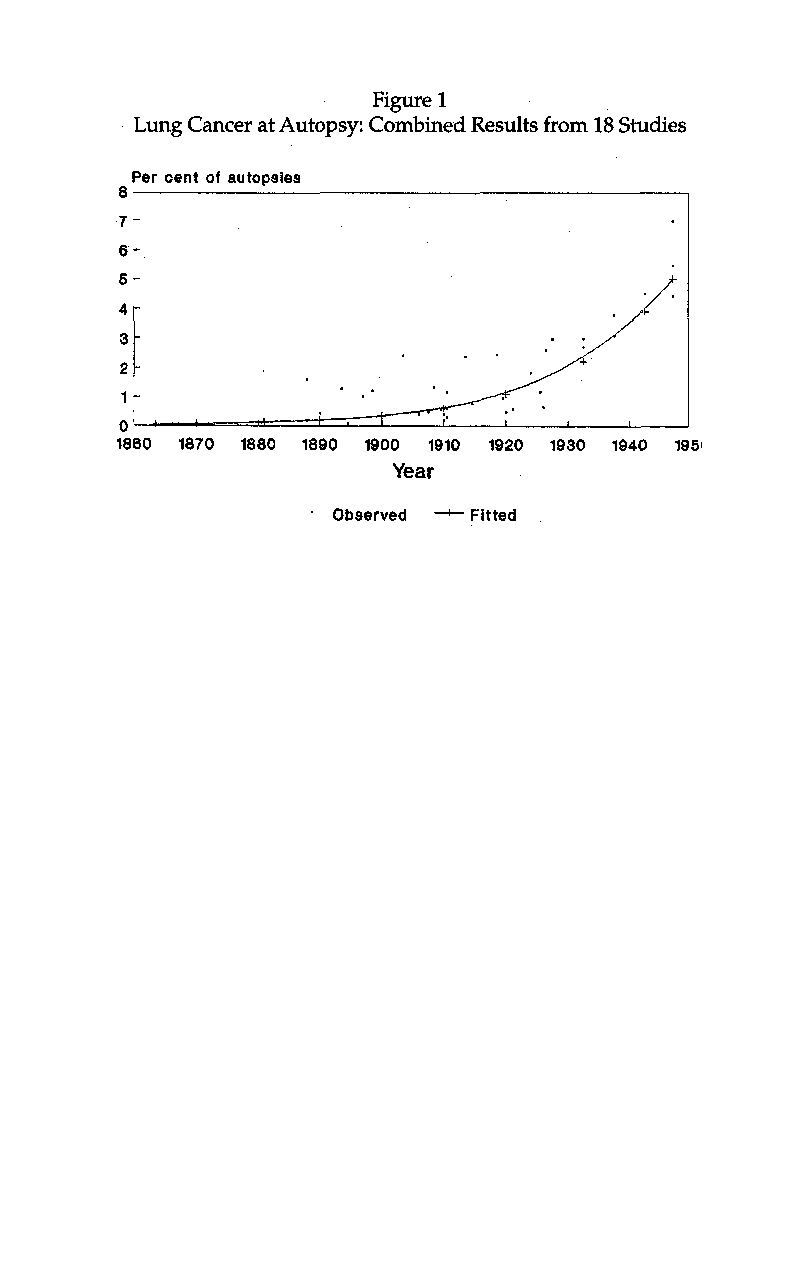
\includegraphics[scale=0.75]{./lecture_includes/cancer_fig1.pdf}
	\end{figure}

	\begin{figure}
	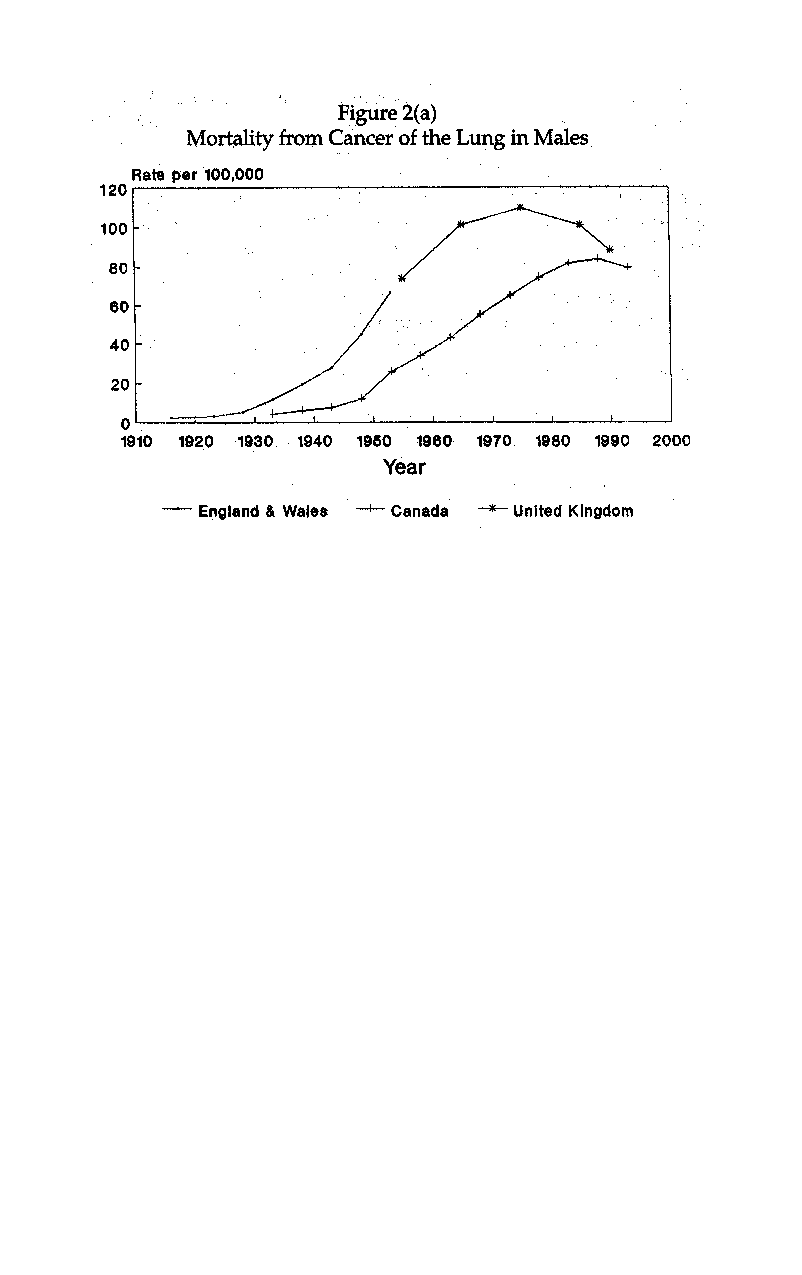
\includegraphics[scale=0.75]{./lecture_includes/cancer_fig2.pdf}
	\end{figure}

\end{frame}	


\begin{frame}[plain]
	
	\begin{figure}
	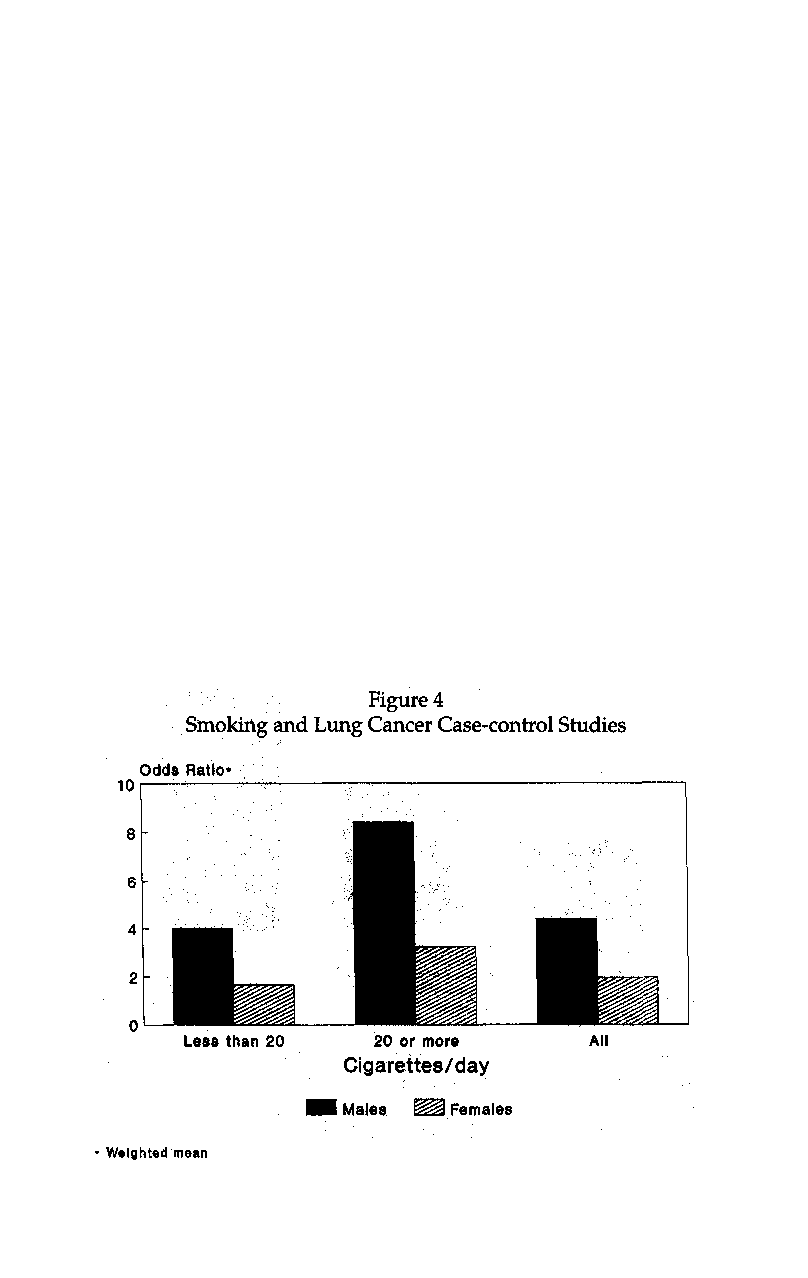
\includegraphics[scale=0.5]{./lecture_includes/smoking_figure1.pdf}
	\end{figure}

	\begin{figure}
	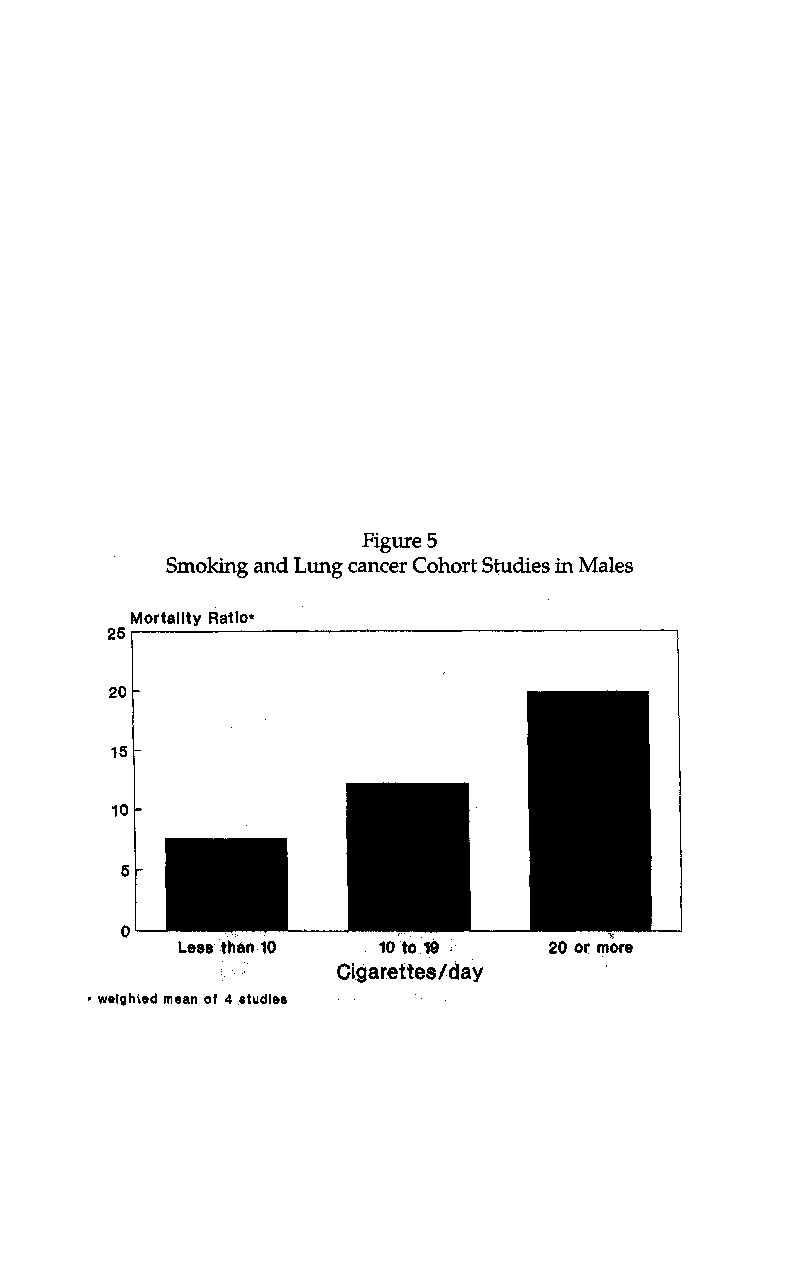
\includegraphics[scale=0.5]{./lecture_includes/smoking_figure2.pdf}
	\end{figure}

\end{frame}	
	

	


\begin{frame}{Hypothesis and skepticism}

Early 20th century scientists believed smoking caused lung cancer but others felt the evidence was not strong
		\begin{enumerate}
		\item Sample bias due to non-random selection of subjects (only those who died)
		\item Complaints about functional forms using ``risk ratios'' and ``odds ratios''
		\item Implausible magnitudes (``smell test'')
		\item Killer critique: \emph{no experimental evidence} to incriminate smoking as a cause of lung cancer
		\end{enumerate}
\end{frame}

\begin{frame}{Fisher's genome confounder theory}
		\begin{itemize}
		\item Ronald Fisher (recall from earlier) was a heavy smoker, died of cancer, and paid expert witness for the tobacco industry
		\item Famous as statistician and as a geneticist and using logic, statistics and genetic evidence proposed a contrarian theory that there existed a confounding genome, $Z$, which introduced selection bias into contrasts of smokers and non-smokers 
		\item Studies showed that cigarette smokers and non-smokers were different on observables -- more extraverted than non-smokers, differed in age, differed in income, differed in education, etc.
		\end{itemize}
\end{frame}

\begin{frame}{Fisher's genome confounder theory in DAG form}
	
Smoking, $S$, is only \emph{correlated} with lung cancer, $C$ because of an unknown ant not quantified confounder $Z$:

  \begin{center}
    \begin{tikzpicture}
    [node distance=1.5cm]

    % nodes %
    \node[text centered] (z) {$Z$};
    \node[below right of = z, text centered] (c) {$C$};
    \node[below left of = z, text centered] (s) {$S$};
    
    % edges %
    \draw[->, line width= 0.5] (z) -- (c);
    \draw[->, line width= 0.5] (z) -- (s);
    % \draw[->, line width= 0.5] (s) -- (c);
    
    \end{tikzpicture}
  \end{center}

Legitimate criticism, but ultimately incorrect:

\bigskip

  \begin{quote}  
    ``the [epidemiologists] turned out to be right, but only because bad logic does not necessarily lead to wrong conclusions.'' Robert Hooke (1983)
  \end{quote}

	
\end{frame}

\begin{frame}{Stratification weighting}

\begin{itemize}
\item Simple weighting techniques were eventually introduced to adjust for these observables
\item Stratification weighting goes back at least to Cochran (1968)
\item We will discuss it both using his original paper, and an application
\item Goal is to adjust quantities for a known and quantified confounder through weights based on the confounder's distribution in different samples
\end{itemize}

\end{frame}




\begin{frame}{Mortality rates by country and smoking group}
	
	\begin{table}\centering
		\caption{Death rates per 1,000 person-years (Cochran 1968)}
		\begin{center}
		\begin{tabular}{lccc}
		\hline \hline
		\multicolumn{1}{l}{Smoking group}&
		\multicolumn{1}{c}{Canada}&
		\multicolumn{1}{c}{U.K.}&
		\multicolumn{1}{c}{U.S.}\\
		\hline
		Non-smokers & 20.2 & 11.3 & 13.5\\
		Cigarettes & 20.5 & 14.1 & 13.5 \\
		Cigars/pipes & 35.5 & 20.7 & 17.4\\
		\hline
		\end{tabular}
		\end{center}
	\end{table}
	
	
\end{frame}

\begin{frame}{Mortality rates by country and smoking group}

\begin{itemize}
\item Cigars in these data are particularly odd to me -- much higher mortality rates in all three countries than non-smokers, as well as cigarette smokers. 
\item Another strange result -- cigarette smokers in Canada and US had same mortality rates as non-smokers
\item Seems weird to us, but unclear what they would've thought given the science was unsettled
\item Cochran tackles \emph{one} of the observable variables that he thinks predicts smoking and mortality -- age

\end{itemize}

\end{frame}


\begin{frame}{Non-smokers and smokers differ in age}
	

	\begin{table}\centering
		\caption{Mean ages, years (Cochran 1968)}
		\begin{center}
		\begin{tabular}{lccc}
		\hline \hline
		\multicolumn{1}{l}{Smoking group}&
		\multicolumn{1}{c}{Canada}&
		\multicolumn{1}{c}{U.K.}&
		\multicolumn{1}{c}{U.S.}\\
		\hline
		Non-smokers & 54.9 & 49.1 & 57.0\\
		Cigarettes & 50.5 & 49.8 & 53.2 \\
		Cigars/pipes & 65.9 & 55.7 & 59.7\\
		\hline
		\end{tabular}
		\end{center}
	\end{table}
	
Maybe age is a confounder. It predicts smoking, but it also predicts mortality as cumulative risk of dying grows as we age
 
\end{frame}

\begin{frame}{Imbalanced confounders and covariates}

\begin{itemize}
\item Balance is a phrase often heard in causal inference -- means treatment and group have different covariate/confounder means and/or distributions
\item If confounders are \emph{imbalanced}, then their means differ in each group, and will introduce selection bias (if confounders, but not if covariates)
\item Weighting, matching and regression that adjust for known and quantified confounders attempt to create balance on confounders and covariates so that their effects stop
\end{itemize}

\end{frame}


\begin{frame}{General description of stratification weighting}
	

\begin{enumerate}
\item[1. ]Stratify the confounder by slicing it into ``strata'' (e.g., age is young vs old)
\item[2. ]Compare quantity of interest across each treatment status within each strata
\item[3. ]Create strata specific weights
\item[4. ]Weight quantity of interest by share of units across all strata
\end{enumerate}

\end{frame}



\begin{frame}{Smoking and stratification weighting}

  \begin{enumerate}
		\item Stratify the smoking group into differing age groups or ``bins'' or ``strata'' (e.g., young and old)
		\item Calculate mortality rates separately for young and old and treatment and control (four averages)
		\item Construct ``probability weights'' as the proportion of each smoking group sample within a given age group
		\item For treatment and control group, compute the weighted averages of the age groups mortality rates using the probability weights
  \end{enumerate}
  
  \bigskip
  
This procedure will balance the observed covariate, age, between treatment and control

\end{frame}


\begin{frame}{Smoking and stratification weighting}
	


	\begin{table}\centering
		\begin{center}
		\begin{tabular}{lccc}
		\hline \hline
		\multicolumn{1}{l}{}&
		\multicolumn{1}{c}{Death rates}&
		\multicolumn{2}{c}{Number of}\\
		\multicolumn{1}{l}{}&
		\multicolumn{1}{c}{Pipe-smokers}&
		\multicolumn{1}{c}{Pipe-smokers}&
		\multicolumn{1}{c}{Non-smokers}\\
		\hline
		Age 20-50 & 15 & 11 & 29 \\
		Age 50-70 & 35 & 13 & 9 \\
		Age $+$70 & 50 & 16 & 2 \\
		Total & & 40 & 40 \\		
		\hline
		\end{tabular}
		\end{center}
	\end{table}
	
	\begin{flalign*}
    \only<1-2>{&\text{Question: Calculate average pipe smoker death rate w/out stratification?}&}\\
    \only<2-2>{&15\cdot\left(\frac{11}{40}\right)+35\cdot\left(\frac{13}{40}\right)+50\cdot\left(\frac{16}{40}\right)=35.5} \\
    \only<3-4>{&\text{Counterfactual question: What would the average mortality rate be for }} \\ 
    \only<3-4>{&\text{pipe smokers if they had the same age distribution as the non-smokers?}}\\
    \only<4-4>{&15\cdot\left(\frac{29}{40}\right)+35\cdot\left(\frac{9}{40}\right)+50\cdot\left(\frac{2}{40}\right)=21.2}
	\end{flalign*}

\end{frame}


\begin{frame}[plain]

	\begin{table}\centering
	\caption{Adjusted death rates using 3 age groups (Cochran 1968)}
		\begin{center}
		\begin{tabular}{lccc}
		\hline \hline
		\multicolumn{1}{l}{Smoking group}&
		\multicolumn{1}{c}{Canada}&
		\multicolumn{1}{c}{U.K.}&
		\multicolumn{1}{c}{U.S.}\\
		\hline
		Non-smokers & 20.2 & 11.3 & 13.5 \\
		Cigarettes & 28.3 & 12.8  &  17.7 \\
		Cigars/pipes & 21.2 & 12.0 & 14.2 \\
		\hline
		\end{tabular}
		\end{center}
	\end{table}

\end{frame}

\begin{frame}{Exercise: Titanic sinking}

\begin{itemize}

\item Titanic sank on maiden voyage April 15, 1912 after hitting an iceberg in North Atlantic
\item 2200 on board, but only 700 survived, despite 20 lifeboats with 60 capacity (1200 potential lives could've been saved)
\item Women and children first was a maritime rule to ration lifeboats, but there were different cabins (1st class, 2nd class, etc.) on different levels with different proximity to boats
\item What was the causal effect of 1st class on survival adjusting for $W$ and $C$?
\end{itemize}

\end{frame}


\begin{frame}{Exercise: Titanic DAG}

\begin{figure}
\begin{center}
\caption{Women $W$ and children $C$ first maritime rule is a confounder for estimating first class $D$ effect on surviving $Y$}
\begin{tikzpicture}[node distance=2cm]
% nodes %
\node[text centered] (d) {$D$};
\node[below left of = d, text centered] (c) {$\mybox{C}$};
\node[above left of = d, text centered] (w) {$\mybox{W}$};
\node[right of = d, text centered] (y) {$Y$};
% edges %
\draw[->, line width= 1] (d) -- (y);
\draw[->, line width= 1] (c) -- (d);
\draw[->, line width= 1] (w) -- (d);
\draw[->, line width= 1] (c) -- (y);
\draw[->, line width= 1] (w) -- (y);
\end{tikzpicture}
\label{fig:titanic}
\end{center}
\end{figure}

\bigskip

Backdoor criterion can be satisfied by blocking on $W$ and $C$.  These are our known confounders.  Now we just need data to see if it's quantified.

\end{frame}

\begin{frame}{Titanic exercise}

\begin{enumerate}
\item \textbf{Stratify the confounders}: Our age and sex variables are both binary, so we can only create four strata: male children, female children, male adults, female adults
\item \textbf{Calculate differences within strata}: Calculate average survival rates for each group within each of the four strata and difference within strata
\item \textbf{Calculate probability weights}: Count the number of people in each strata and divide by the total number of souls aboard (crew and passengers)
\item \textbf{Aggregate differences across strata using weights}: Estimate the ATE by aggregating the difference in survival rates over the four strata with each strata-specific difference weighted by that strata's weight
\end{enumerate}

\bigskip

Go to lab

\end{frame}

\begin{frame}{Table 1: Simple counts}

{\renewcommand{\arraystretch}{1.1}
\tabcolsep=1.3\tabcolsep 		
\begin{table}\small\index{rolling!3}
\caption{Differences in female and adult passengers by first class status on the Titanic. }
\centering
\begin{tabular}{lcc|cc}
\toprule
\multicolumn{1}{c}{\textbf{Variable name}}&
\multicolumn{2}{c}{\textbf{First class}}&
\multicolumn{2}{c}{\textbf{All other classes}}\\
\multicolumn{1}{c}{}&
\multicolumn{1}{c}{Obs}&
\multicolumn{1}{c}{Mean}&
\multicolumn{1}{c}{Obs}&
\multicolumn{1}{c}{Mean}\\
\midrule
Percent adult		&	325 	& 98.2\% & 1,876 & 94.5\% \\
Percent female		& 	325	& 44.6\% & 1,876 & 17.3\% \\
\bottomrule
\end{tabular}
\label{tab:titanic-age}
\end{table}}
\end{frame}


\begin{frame}{Table 2: Stratified sample}

{\renewcommand{\arraystretch}{1.1}
\tabcolsep=1.3\tabcolsep 		
\begin{table}\small\index{rolling!3}
\caption{Counts and Titanic survival rates by strata and first class status.}
\centering
\begin{tabular}{lcc|cc|c}
\toprule
\multicolumn{1}{c}{\textbf{}}&
\multicolumn{2}{c}{\textbf{First class}}&
\multicolumn{2}{c}{\textbf{All other classes}}&
\multicolumn{1}{c}{\textbf{}}\\
\multicolumn{1}{l}{Strata}&
\multicolumn{1}{c}{Obs}&
\multicolumn{1}{c}{Mean}&
\multicolumn{1}{c}{Obs}&
\multicolumn{1}{c}{Mean}&
\multicolumn{1}{c}{Total}\\
\midrule
Male adult		& 175	& 0.326	& 1,492	& 0.188	& 1,667 \\
Female adult	& 144	& 0.972	& 281	& 0.626	& 425 \\
Male child		& 5		& 1		& 59		& 0.407 	& 64\\
Female child	& 1		& 1		& 44		& 0.613 	& 45\\
\midrule
Total	observations	& 325	&&	1,876	 && 2,201\\
\bottomrule
\end{tabular}
\label{tab:titanic-counts}
\end{table}}


\end{frame}

\begin{frame}{Table 3: Estimates of aggregate parameter}

{\renewcommand{\arraystretch}{1.1}
\tabcolsep=1.3\tabcolsep 		
\begin{table}\tiny\index{rolling!3}
\caption{Differences in survival rates, stratification weights, and estimates of parameters}
\centering
\begin{tabular}{lc|ccc}
\toprule
\multicolumn{1}{l}{\textbf{Strata}}&
\multicolumn{1}{c}{\textbf{Differences in Survival Rates}}&
\multicolumn{1}{c}{\textbf{Weight$_{k,ATE}$}}&
\multicolumn{1}{c}{\textbf{Weight$_{k,ATT}$}}&
\multicolumn{1}{c}{\textbf{Weight$_{k,ATU}$}}\\
\midrule
Male adult		& 0.138 &	0.76 &	0.54	&0.80	\\
Female adult	& 0.346 &	0.19 &	0.44	&0.15	\\
Male child		& 0.593 &	0.03 &	0.02	&0.03	\\
Female child	& 0.387 &	0.02 &	0.00	&0.02	\\
\midrule
\multicolumn{1}{l}{\textbf{}}&
\multicolumn{1}{c}{\textbf{No stratification}}&
\multicolumn{3}{c}{\textbf{Stratification weighted estimates}}\\

 & $\widehat{\textbf{SDO}}$& $\widehat{\textbf{ATE}}$ & $\widehat{\textbf{ATT}}$ & $\widehat{\textbf{ATU}}$ \\
\midrule
\textbf{Estimated coefficient}& 0.35 & 0.20 & 	0.24	 & 0.19   \\
\bottomrule
\end{tabular}
\label{tab:titanic-weights}
\end{table}}

\end{frame}

\begin{frame}{Drop the one female child}

\begin{itemize}
\item We were able to estimate all three causal effect parameters because for all four strata there were units in both treatment and control
\item But if we dropped the only female child in first class from the data, we'd be in trouble bc there wouldn't be any way to calculate a difference for that group
\item But what could we identify?

\end{itemize}

\end{frame}

\begin{frame}

\begin{table}\tiny\index{rolling!3}
\caption{Counts and Titanic survival rates by strata and first class status.}
\centering
\begin{tabular}{lcc|cc|c}
\toprule
\multicolumn{1}{c}{\textbf{}}&
\multicolumn{2}{c}{\textbf{First class}}&
\multicolumn{2}{c}{\textbf{All other classes}}&
\multicolumn{1}{c}{\textbf{}}\\
\multicolumn{1}{l}{Strata}&
\multicolumn{1}{c}{Obs}&
\multicolumn{1}{c}{Mean}&
\multicolumn{1}{c}{Obs}&
\multicolumn{1}{c}{Mean}&
\multicolumn{1}{c}{Total}\\
\midrule
Male adult		& 175	& 0.326	& 1,492	& 0.188	& 1,667 \\
Female adult	& 144	& 0.972	& 281	& 0.626	& 425 \\
Male child		& 5		& 1		& 59		& 0.407 	& 64\\
Female child	& 0		& n/a		& 44		& 0.613 	& 44\\
\midrule
Total	observations	& 324	&&	1,876	 && 2,200\\
\bottomrule
\end{tabular}
\label{tab:titanic-counts2}
\end{table}

\end{frame}

\begin{frame}{ATT is the only one we can get}

\begin{eqnarray}
\widehat{\delta}_{ATT} &=& (0.137 \times 0.54) + (0.346 \times 0.44) + (0.593 \times 0.02)  \nonumber \\
&=& 0.24\text{ or 24 percentage points}
\end{eqnarray}

\end{frame}

\begin{frame}

\begin{table}\tiny\index{rolling!3}
\caption{Differences in survival rates, stratification weights, and estimates of parameters without perfect stratification}
\centering
\begin{threeparttable}
\begin{tabular}{lc|ccc}
\toprule
\multicolumn{1}{l}{\textbf{Strata}}&
\multicolumn{1}{c}{\textbf{Differences in Survival Rates}}&
\multicolumn{1}{c}{\textbf{Weight$_{k,ATE}$}}&
\multicolumn{1}{c}{\textbf{Weight$_{k,ATT}$}}&
\multicolumn{1}{c}{\textbf{Weight$_{k,ATU}$}}\\
\midrule
Male adult		& 0.137 	&	0.76 &	0.54	&0.80	\\
Female adult	& 0.346 	&	0.19 &	0.44	&0.15	\\
Male child		& 0.593 	&	0.03 &	0.02	&0.03	\\
Female child	& n/a 	&	n/a 	&	n/a	&0.02	\\
\midrule
\multicolumn{1}{l}{\textbf{}}&
\multicolumn{1}{c}{\textbf{No stratification}}&
\multicolumn{3}{c}{\textbf{Stratification weighted estimates}}\\

 & $\widehat{\textbf{SDO}}$& $\widehat{\textbf{ATE}}$ & $\widehat{\textbf{ATT}}$ & $\widehat{\textbf{ATU}}$ \\
\midrule
\textbf{Estimated coefficient}& 0.35 & n/a & 	0.24	 & n/a  \\
\bottomrule
\end{tabular}
\begin{tablenotes}
\tiny
\item 
Differences in survival rates, stratification weights, and estimated parameters. All coefficients should be multiplied by 100 to get a percentage point change in survival rate as a result of having a first class cabin. Note that the SDO is a simple difference in mean outcomes and therefore \emph{not} a weighted average over the strata differences.  But the estimated ATE, ATT and ATU parameters are weighted averages in difference in means using corresponding stratification weights. 
\end{tablenotes}
\end{threeparttable}
\label{tab:titanic-weights2}
\end{table}


\end{frame}

\begin{frame}{Why did this happen?}

\begin{itemize}

\item Stratification requires having units in both groups for every value of $X$ to get ATE
\item If you want the ATT, you have to have units in the control group for every treated group based on its value of $X$ (female children weren't treated, so didn't matter)
\item If you want the ATU, you have to have units in the treatment group for every treated group based on its value of $X$ (female children weren't treated, so did matter)
\item This has a technical word we are going to learn more about called a ``lack of common support''
\end{itemize}

\end{frame}

\subsection{Conditional Independence}

\begin{frame}{Potential outcomes}

\begin{itemize}
\item Now let's introduce potential outcomes notation so that we can build more formalized models
\item This helps us understand what assumptions we need to make, which is not necessarily spelled out in the DAG backdoor criterion
\end{itemize}

\end{frame}

\begin{frame}{Recall the RCT Assumption of Independence}
	
	\begin{itemize}
	\item Randomized treatment assignment guarantees ``independence'' $$(Y^0,Y^1)\independent{D}$$
	\item Independence allows to estimate accurate causal effects through simple methods like differences in averages
		\begin{eqnarray*}
		E[Y|D=1] - E[Y|D=0] &=& \underbrace{E[Y^1|D=1] - E[Y^0|D=0]}_{\mathclap{\text{by the switching equation}}} \\
		&=& \underbrace{E[Y^1] - E[Y^0]}_{\mathclap{\text{by independence}}} \\
		&=& \underbrace{E[Y^1-Y^0]}_{\mathclap{\text{ATE}}}
		\end{eqnarray*}
	\end{itemize}
\end{frame}

\begin{frame}{Confounder and covariate distribution}

\begin{itemize}
\item Just like independence implies balance on expected potential outcomes, it also implies balance on confounders and covariates which is called ``common support''
\item We saw this in our Thornton regressions: cash vouchers were not associated with being male, one's age, etc.
\item If we have balance on potential outcomes, that's all we need but as that's not observed, balance on covariates is often used to provide some evidence the randomization was done well
\end{itemize}
\end{frame}

\begin{frame}{Violations of independence}

\begin{itemize}
\item Problem with smoking and cancer was smoking wasn't \emph{randomly assigned} -- it was chosen by the ``perfect doctor'' (i.e., self selection into smoking based on factors related to potential outcomes)
\item When a treatment is ``dependent'' on potential outcomes, it means people smoke because they expect something is better when they smoke ($Y^1$) than when they don't ($Y^0$) introducing selection bias and potentially heterogenous treatment effect bias
\item Naive comparisons can be deeply misleading -- covariate adjustment can resolve this if ``conditional independence'' happens in the data
\item How do we express backdoor criterion using potential outcomes notation?
\end{itemize}

\end{frame}



\begin{frame}[plain]

	\begin{block}{Identifying assumption I: Conditional independence}
	$(Y_i^0$, $Y_i^1)$ $\independent{D} | X_i$. There exists a set $X$ of known and quantified confounders such that after adjusting for them, treatment assignment is \emph{independent of potential outcomes}.
	\end{block}
	
	\begin{itemize}
	\item Conditional on $X$, treatment assignment is \textbf{random}
	\item For a large group of people within the same strata, they flipped coins as opposed to sought treatments that helped them
	\item Sometimes this is called also ``unconfoundedness'' and worth thinking long and hard about
	\end{itemize}
\end{frame}


\begin{frame}[plain]

	\begin{block}{Identifying assumption I: Conditional independence}
	$(Y_i^0$, $Y_i^1)$ $\independent{D} | X_i$. There exists a set $X$ of known and quantified confounders such that after adjusting for them, treatment assignment is \emph{independent of potential outcomes}.
	\end{block}
	
	\begin{eqnarray*}
	E[Y^0 | D=1, X=x] &=& E[Y^0 | D=0, X=x] \\
	E[Y^1 | D=1, X=x] &=& E[Y^1 | D=0, X=x] 
	\end{eqnarray*}
	
	Allows us to write down these equalities, which means we can use comparison units as substitutes for counterfactuals so long as there exist one-to-one within $X=x$, leading to our next assumption -- common support
	
\end{frame}



\begin{frame}[plain]

	\begin{block}{Identifying assumption II: Common support}
	For ranges of $X$, there is a positive probability of being both treated and untreated
	\end{block}
	
	\begin{itemize}
	\item There exists units in treatment and control with same values of $X$
	\item Dimension $k$ means every specific combination of the conditioning set (e.g., not males and old, but adult males, adult females, youth male, youth female)
	\item Testable, and often this is where regression steps don't incorporate it
	\end{itemize}
	
	
\end{frame}



\begin{frame}{Caveat: Perfect Doctor and conditional independence}

\begin{itemize}
\item Independence was violated if the treatment was assigned \emph{because} we expected things to improve or not (``perfect doctor'' reasoning)
\item If you take an action because you think it helps and others don't take the action because they don't or can't, then it is a violation of independence probably
\item For a large group of people within the same strata, they flipped coins as opposed to sought treatments that helped them
\item Rationality is contained in the confounders -- worth reflecting a lot on
\end{itemize}

\end{frame}


\begin{frame}{Assumptions combined}
	
We need only two assumptions to estimate the ATE, but these are not trivial: 
  \begin{enumerate}
		\item $(Y^1,Y^0) \independent{D} | X$ (conditional independence)
		\item $0<Pr(D=1|X)<1$ with probability one (common support)
  \end{enumerate}

\bigskip
Comparing groups of individuals \emph{who have the same values of} $X$, treatment is no longer based gains, $\delta$. 

\bigskip

The second term implies we have people in treatment and control for every strata of $X$
\end{frame}


\begin{frame}{Implications of assumptions}


	\begin{itemize}
	\item Assumption 1 lets you plug $Y$ for $Y^j$ with the switching equation
		\begin{eqnarray*}
		E[Y^1-Y^0|X] &=& E[Y^1 - Y^0 | X,D=1] \\
		&=&E[Y|X,D=1] - E[Y|X,D=0]
		\end{eqnarray*}
	\item Assumption 2 lets you weight over the covariate distribution
		\begin{eqnarray*}
		\delta_{ATE} &=&E[Y^1-Y^0] = E\bigg[ E[Y^1 - Y^0 \ \vert \ X] \bigg] \\
		&=& \int E[Y^1 - Y^0 |X,D=1] dPr(X) \\
		&=& \int \left(E[Y|X,D=1] - E[Y|X,D=0]\right)dPr(X)
		\end{eqnarray*}
	\end{itemize}

\end{frame}




\begin{frame}{You need fewer assumptions for ATT or ATU}

Other versions of conditional independence

\begin{enumerate}
  \item $Y^0 \independent{D} | X$ 
  \item $Pr(D=1|X)<1$ (with $Pr(D=1)>0$)
\end{enumerate}

\bigskip
Notice how there is only one potential outcome in the independence equation.  That's okay.  We can still then estimate the ATT (just not the ATE).

\end{frame}



\begin{frame}{Summarizing}


Weighted averages under either assumption:
		\begin{eqnarray*}
		\delta_{ATE} &=& \int \left(E[Y|X,D=1] - E[Y|X,D=0]\right)dPr(X) \\
		\delta_{ATT} &=& \int \left(E[Y|X,D=1] - E[Y|X,D=0]\right)dPr(X|D=1)
		\end{eqnarray*}
ATE needs independence with respect to both potential outcomes; ATT only needs it with respect to $Y^0$. 		
		
\end{frame}

\begin{frame}{Review stratification weighting in light of this}

\begin{itemize}

\item Let's now look at the way in this works within stratification if we are missing some observations
\item The reason that this happens is because the dimensions $K$ of the $X$ conditioning set is getting larger

\end{itemize}

\end{frame}

\begin{frame}{Weighting by Age ($K=2$)}
	
	\begin{table}\centering
		\begin{center}
		\begin{tabular}{lccccc}
		\hline \hline
		\multicolumn{1}{l}{}&
		\multicolumn{2}{c}{Death Rate}&
		\multicolumn{1}{c}{}&
		\multicolumn{2}{c}{Number of}\\

		\multicolumn{1}{l}{$X_k$}&
		\multicolumn{1}{c}{Smokers}&
		\multicolumn{1}{c}{Non-smokers}&
		\multicolumn{1}{c}{Diff.}&
		\multicolumn{1}{c}{Smokers}&
		\multicolumn{1}{c}{Non-smokers}\\
		\hline
		Old & 28 & 24 & 4 & 3 & 10 \\
		Young & 22 & 16 & 6 & 7 & 10 \\
		Total & & & & 10 & 20 \\
		\hline
		\end{tabular}
		\end{center}
	\end{table}
	
	

	\begin{flalign*}
		    \only<1-2>{&\text{Question: What is $\widehat{\delta_{ATE}}=\sum_{k=1}^K(\overline{Y}^{1,k} - \overline{Y}^{0,k})\cdot \left(\frac{N^k}{N}\right)$?}&}\\
		    \only<2-2>{&4\cdot\left(\frac{13}{30}\right)+6\cdot\left(\frac{17}{30}\right)=5.13} \\
		    \only<3-4>{&\text{Question: What is $\widehat{\delta_{ATT}}=\sum_{k=1}^K(\overline{Y}^{1,k} - \overline{Y}^{0,k})\cdot \left(\frac{N^k_T}{N_T}\right)$?}} \\ 
		    \only<4-4>{&4\cdot\left(\frac{3}{10}\right)+6\cdot\left(\frac{7}{10}\right)=5.4} 
	\end{flalign*}

\end{frame}
	
		
 

\begin{frame}[shrink=20,plain]{Weighting by Age and Gender ($K=4$)}
	
	\begin{table}\centering
		\begin{center}
		\begin{tabular}{lccccc}
		\hline \hline
		\multicolumn{1}{l}{}&
		\multicolumn{2}{c}{Death Rate}&
		\multicolumn{1}{c}{}&
		\multicolumn{2}{c}{Number of}\\

		\multicolumn{1}{l}{$X_k$}&
		\multicolumn{1}{c}{Smokers}&
		\multicolumn{1}{c}{Non-smokers}&
		\multicolumn{1}{c}{Diff.}&
		\multicolumn{1}{c}{Smokers}&
		\multicolumn{1}{c}{Non-smokers}\\
		\hline
		Old Males & 28 & 22 & 4 & 3 & 7 \\
		Old Females &   & 24 &   &   & 3 \\
		Young Males & 21 & 16 & 5 & 3 & 4 \\
		Young Females & 23 & 17 & 6 & 4 & 6 \\
		Total & & & & 10 & 20 \\
		\hline
		\end{tabular}
		\end{center}
	\end{table}
	
	

	\begin{flalign*}
		    \only<1-2>{&\text{Problem: What is $\widehat{\delta_{ATE}}=\sum_{k=1}^K(\overline{Y}^{1,k} - \overline{Y}^{0,k})\cdot \left(\frac{N^k}{N}\right)$?}&}\\
		    \only<2-2>{&\text{Not identified! What went wrong?}} \\
		    \only<3-4>{&\text{Question: What is $\widehat{\delta_{ATT}}=\sum_{k=1}^K(\overline{Y}^{1,k} - \overline{Y}^{0,k})\cdot \left(\frac{N^k_T}{N_T}\right)$?}} \\ 
		    \only<4-4>{&4\cdot\left(\frac{3}{10}\right)+5\cdot\left(\frac{3}{10}\right)+6\cdot\left(\frac{4}{10}\right)=5.1}
	\end{flalign*}

\end{frame}

\begin{frame}{Curse of Dimensionality}
	
	\begin{itemize}
	\item Stratification methods, including OLS, may become less feasible in finite samples as the number of covariates grows (e.g., $K=4$ was too many for this sample)
	\item Assume we have $k$ covariates and we divide each into 3 coarse categories (e.g., age: young, middle age, old; income: low, medium, high, etc.)
	\item The number of strata is $3^k$. For $k=10$, then it's $3^{10}=59,049$
	\item The problem isn't just the number of covariates; it's the number of strata based on those covariates (you can hit the curse fast)
	\end{itemize}
\end{frame}

\begin{frame}{Curse of Dimensionality}
	
	\begin{itemize}
	\item If sparseness occurs, it means many cells may contain either only treatment units or only control units but not both, and that violates our second assumption
	\item We can always use ``finer'' classifications, but finer cells worsens the dimensional problem, so we don't gain  much from that.  ex: using $10$ variables and $5$ categories for each, we get $5^{10} = 9,765,625$.  
	\item Matching methods really force us to see these curses; they're often hidden from OLS because OLS doesn't tell us it is just doing various extrapolations
	\item Simple weighting methods is also a problem if the cells are ``too coarse''
	\end{itemize}
\end{frame}	


\subsection{Exact matching}

\begin{frame}{Exact matching}

\begin{figure}[!t]\centering
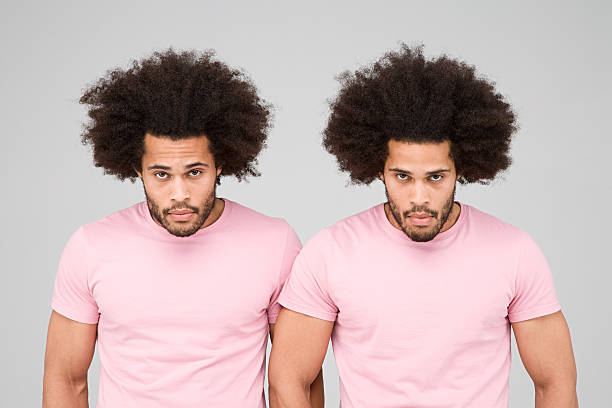
\includegraphics[scale=1.1]{./lecture_includes/identical_twins}
\end{figure}

\end{frame}

\begin{frame}{Quote from Imbens and Rubin 2015}

\begin{quote}
``At some level, all methods for causal inference can be viewed as imputation methods, although some more explicitly than others.''
\end{quote}

\bigskip

Stratification weighting doesn't exactly always help you see the imputation -- where you literally ``fill in'' missing counterfactuals either through estimating them or simply plug-in, but matching does

\bigskip

Matching will match a treated unit to a comparison unit that is similar (or in exact matching identical) on a known and quantified confounder



\end{frame}

\begin{frame}{ATE estimator}

We can estimate the ATE using matching, but we need exact matches on both sides -- and therefore full conditional independence

\bigskip

\begin{equation}
\widehat{\delta}_{ATE} = \dfrac{1}{N} \sum_{i=1}^N (2D_i - 1) \bigg [ Y_i - \bigg ( \dfrac{1}{M} \sum_{m=1}^M Y_{j_m(i)} \bigg ) \bigg ]
\label{eq:ate_match}
\end{equation}

\bigskip

I'm going to just stick with the ATT

\end{frame}


\begin{frame}{ATT estimator}

Equation for ATT estimator is:

\begin{equation}
\widehat{\delta}_{ATT} = \dfrac{1}{N_T} \sum_{D_i=1}(Y_i - Y_{j(i)})
\label{eq:att_simplematch}
\end{equation}

where $Y_{j(i)}$ is the $j$\textsuperscript{th} unit matched to the $i$\textsuperscript{th} unit based on the $j$\textsuperscript{th} being ``exactly equal to'' the $i$\textsuperscript{th} unit with respect to the $X$ conditioning set

\end{frame}

\begin{frame}{Number of matches}

What if I find two or more $M$ units with the identical $X$ value? Then what?

\begin{equation}
\widehat{\delta}_{ATT} = \dfrac{1}{N_T} \sum_{D_i=1} \bigg ( Y_i - \bigg [\dfrac{1}{M} \sum_{m=1}^M Y_{j_m(1)} \bigg ] \bigg )
\label{eq:att_match}
\end{equation}

\bigskip

Notice that we are only dealing with $Y^0_i$ by matching; The $Y^1_i$ is fine as is.

\end{frame}

\begin{frame}{Training example (unmatched)}

{\renewcommand{\arraystretch}{1.1}
\tabcolsep=2.5\tabcolsep
\begin{table}[htb]\tiny\index{rolling!3}
\centering
\begin{tabular}{ccc|ccc}
\toprule
	\multicolumn{3}{c}{\textbf{Trainees}}&
	\multicolumn{3}{c}{\textbf{Non-Trainees}}\\
	\multicolumn{1}{c}{Unit}&
	\multicolumn{1}{c}{Age}&
	\multicolumn{1}{c}{Earnings}&
	\multicolumn{1}{c}{Unit}&
	\multicolumn{1}{c}{Age}&
	\multicolumn{1}{c}{Earnings}\\
\midrule
1 & 	31 & \$	26,629 & 	1 & 	29 & \$	23,178 \\
2 & 	31 & \$	26,633 & 	2 & 	39 &\$ 	33,817 \\
3 & 	18 & 	\$	15,324 & 	3 & 	33 & \$	27,061 \\
4 & 	32 &\$ 	27,717 & 	4 & 	46 & \$	43,109 \\
5 & 	32 & \$	27,725 & 	5 & 	32 & \$	26,040 \\
6 & 	25 & \$	20,762 & 	6 & 	39 & \$	33,815 \\
7 & 	32 &\$ 	27,716 & 	7 & 	31 & \$	25,052 \\
8 & 	32 & \$	27,719 & 	8 & 	33 & \$	27,060 \\
9 & 	20 & \$	16,723 & 	9 & 	25 &\$ 	19,787 \\
10 & 	29 & \$	24,552 & 	10 & 	29 &\$ 	23,173 \\
&&&			11 & 	27 & 	21,416 \\
&&&			12 & 	32 & 	26,040 \\
&&&			13 & 	20 & 	16,246 \\
&&&			14 & 	41 & 	36,316 \\
&&&			15 & 	18 & 	15,046 \\
&&&			16 & 	29 & 	23,178 \\
&&&			17 & 	49 & 	47,559 \\
&&&			18 & 	32 & 	26,040 \\
&&&			19 & 	27 & 	21,418 \\
&&&			20 & 	46 & 	43,109 \\
\midrule
Mean & 	28.2 & 	\$24,150 & 	Mean & 	32.85 & 	\$27,923 \\
\bottomrule
\end{tabular}
\label{tab:trainee1}
\end{table}
}

\end{frame}

\begin{frame}{SDO}

\begin{equation}
SDO = \$24,150-27,923 = -\$3,773
\end{equation}

\end{frame}


\begin{frame}{Age Imbalance}

\begin{figure}[!t]\centering
\caption{Age distribution of a job training program's trainees (figure a) versus a sample of workers who were not enrolled in the trainee program (figure b).}
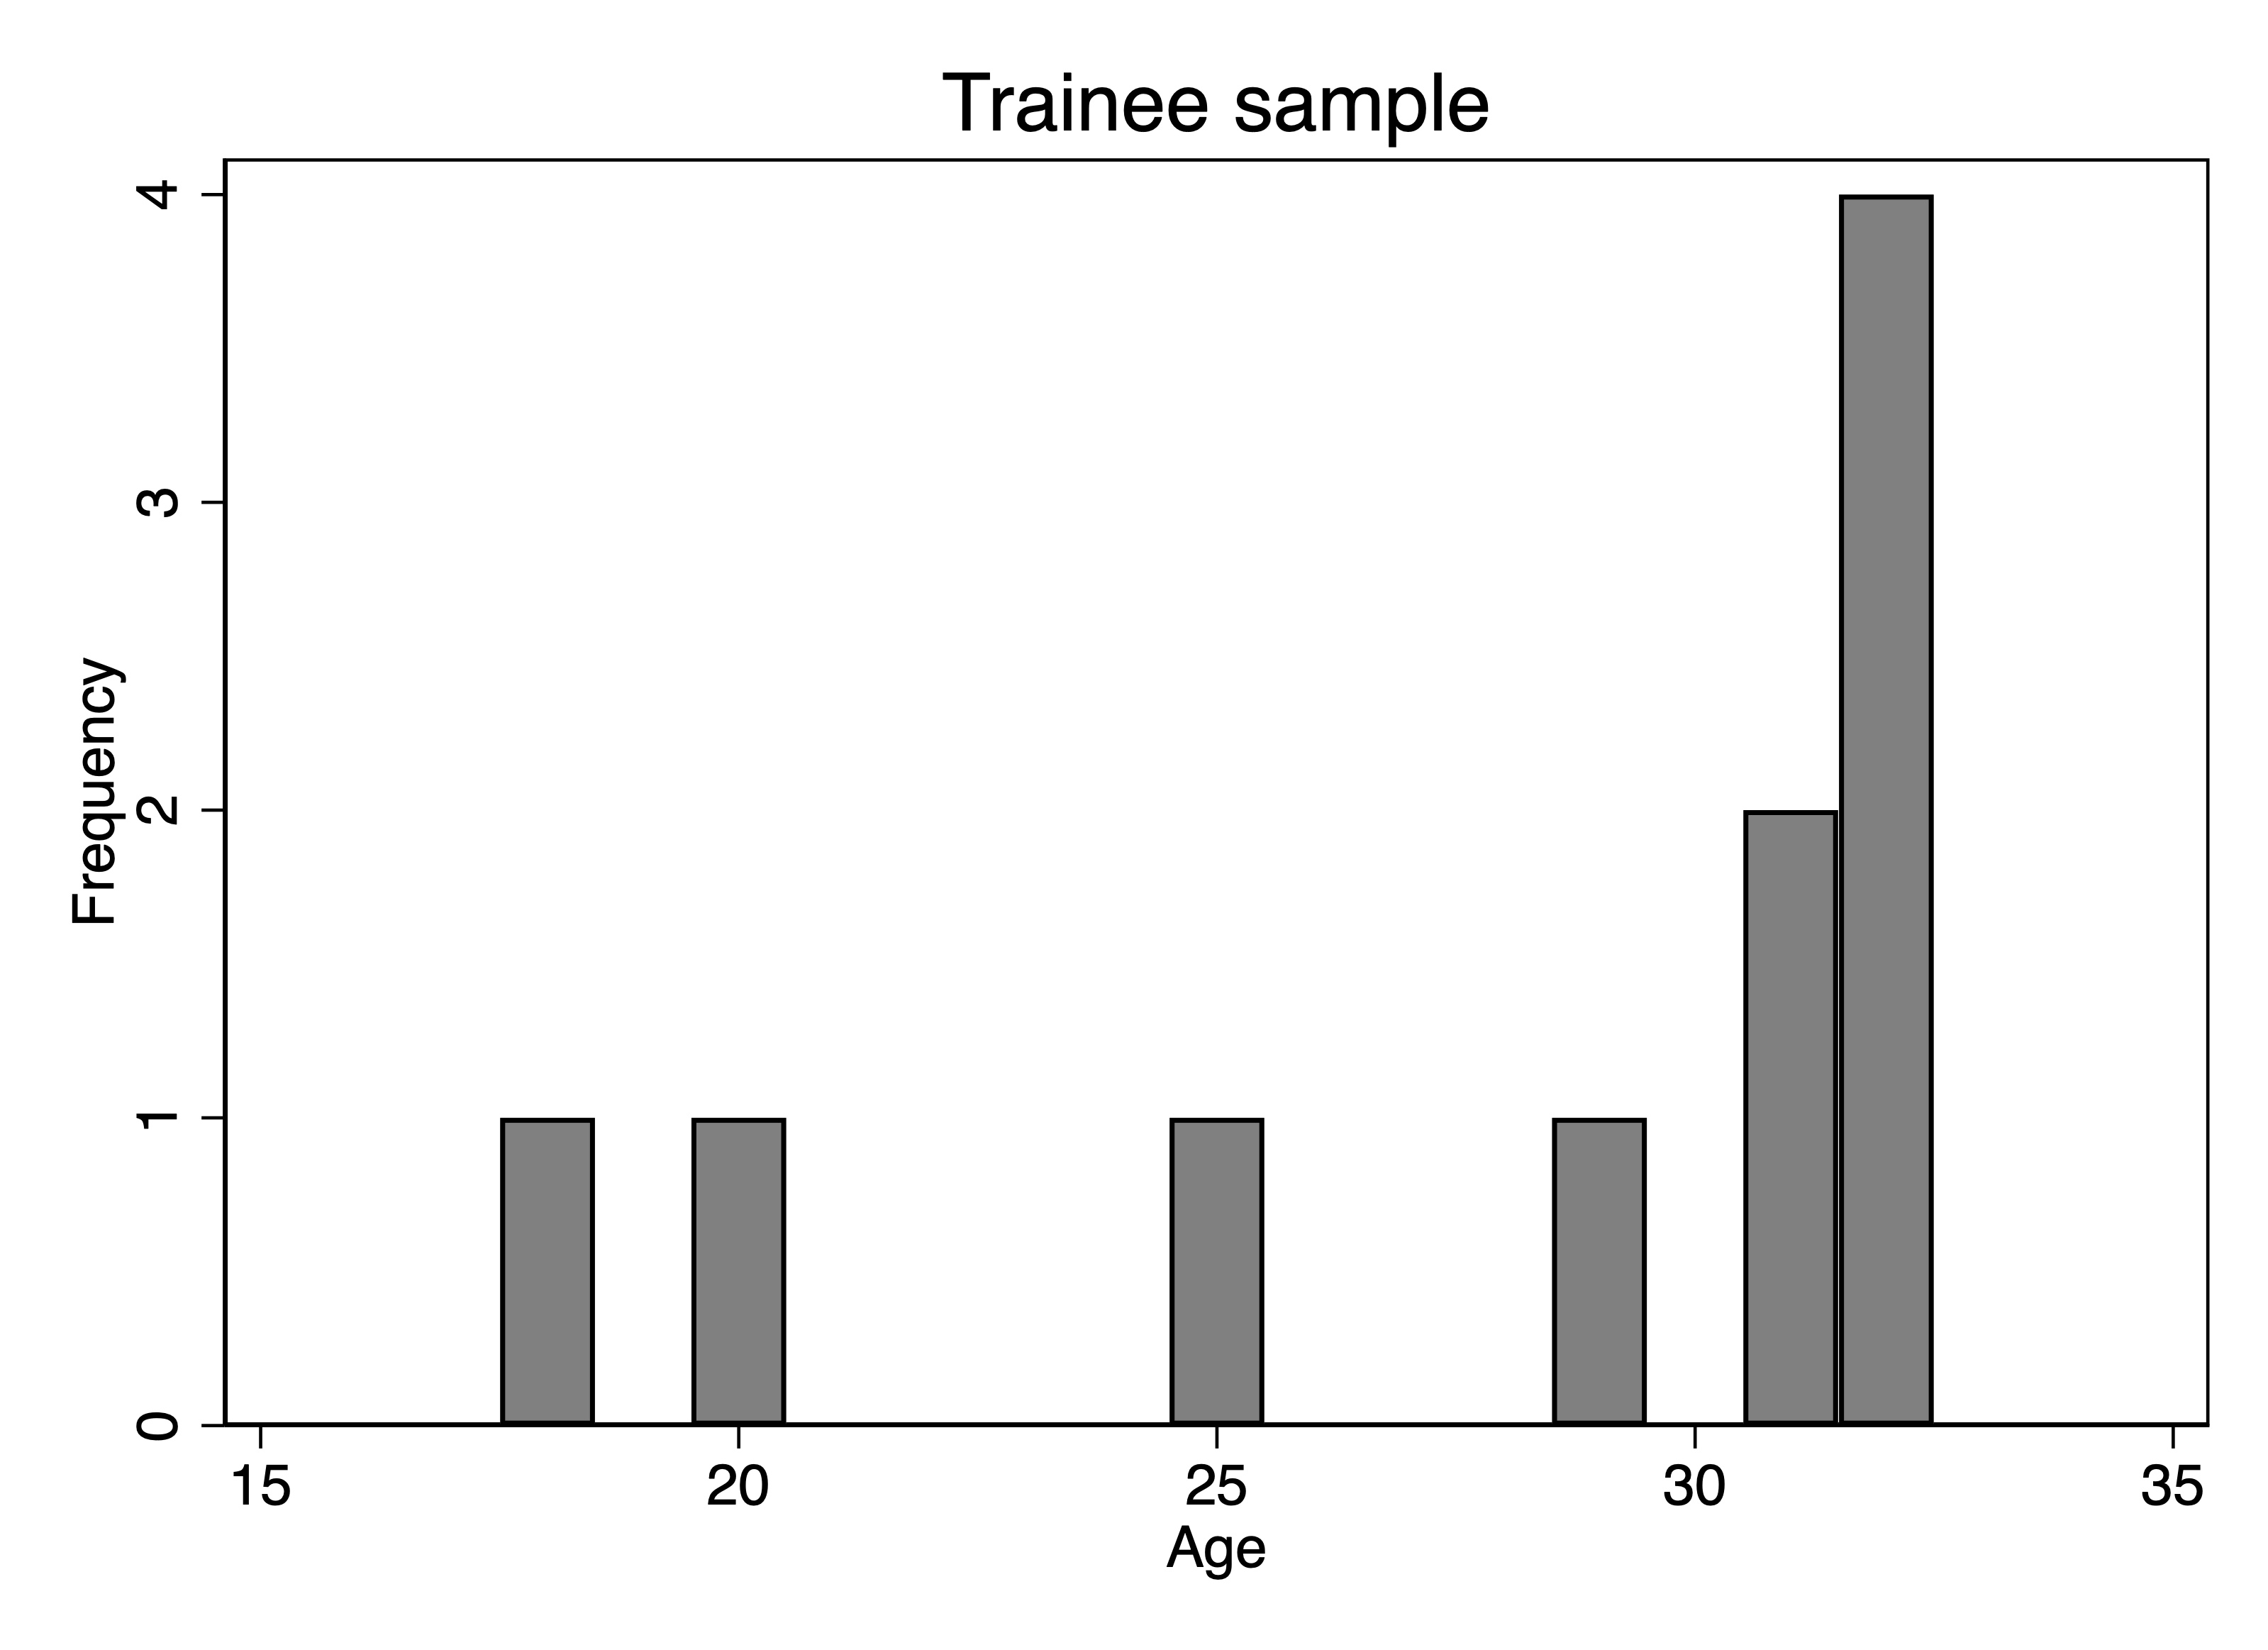
\includegraphics[scale=0.075]{./lecture_includes/trainees.jpg}
\end{figure}

\end{frame}

\begin{frame}{Age Imbalance}

\begin{figure}[!t]\centering
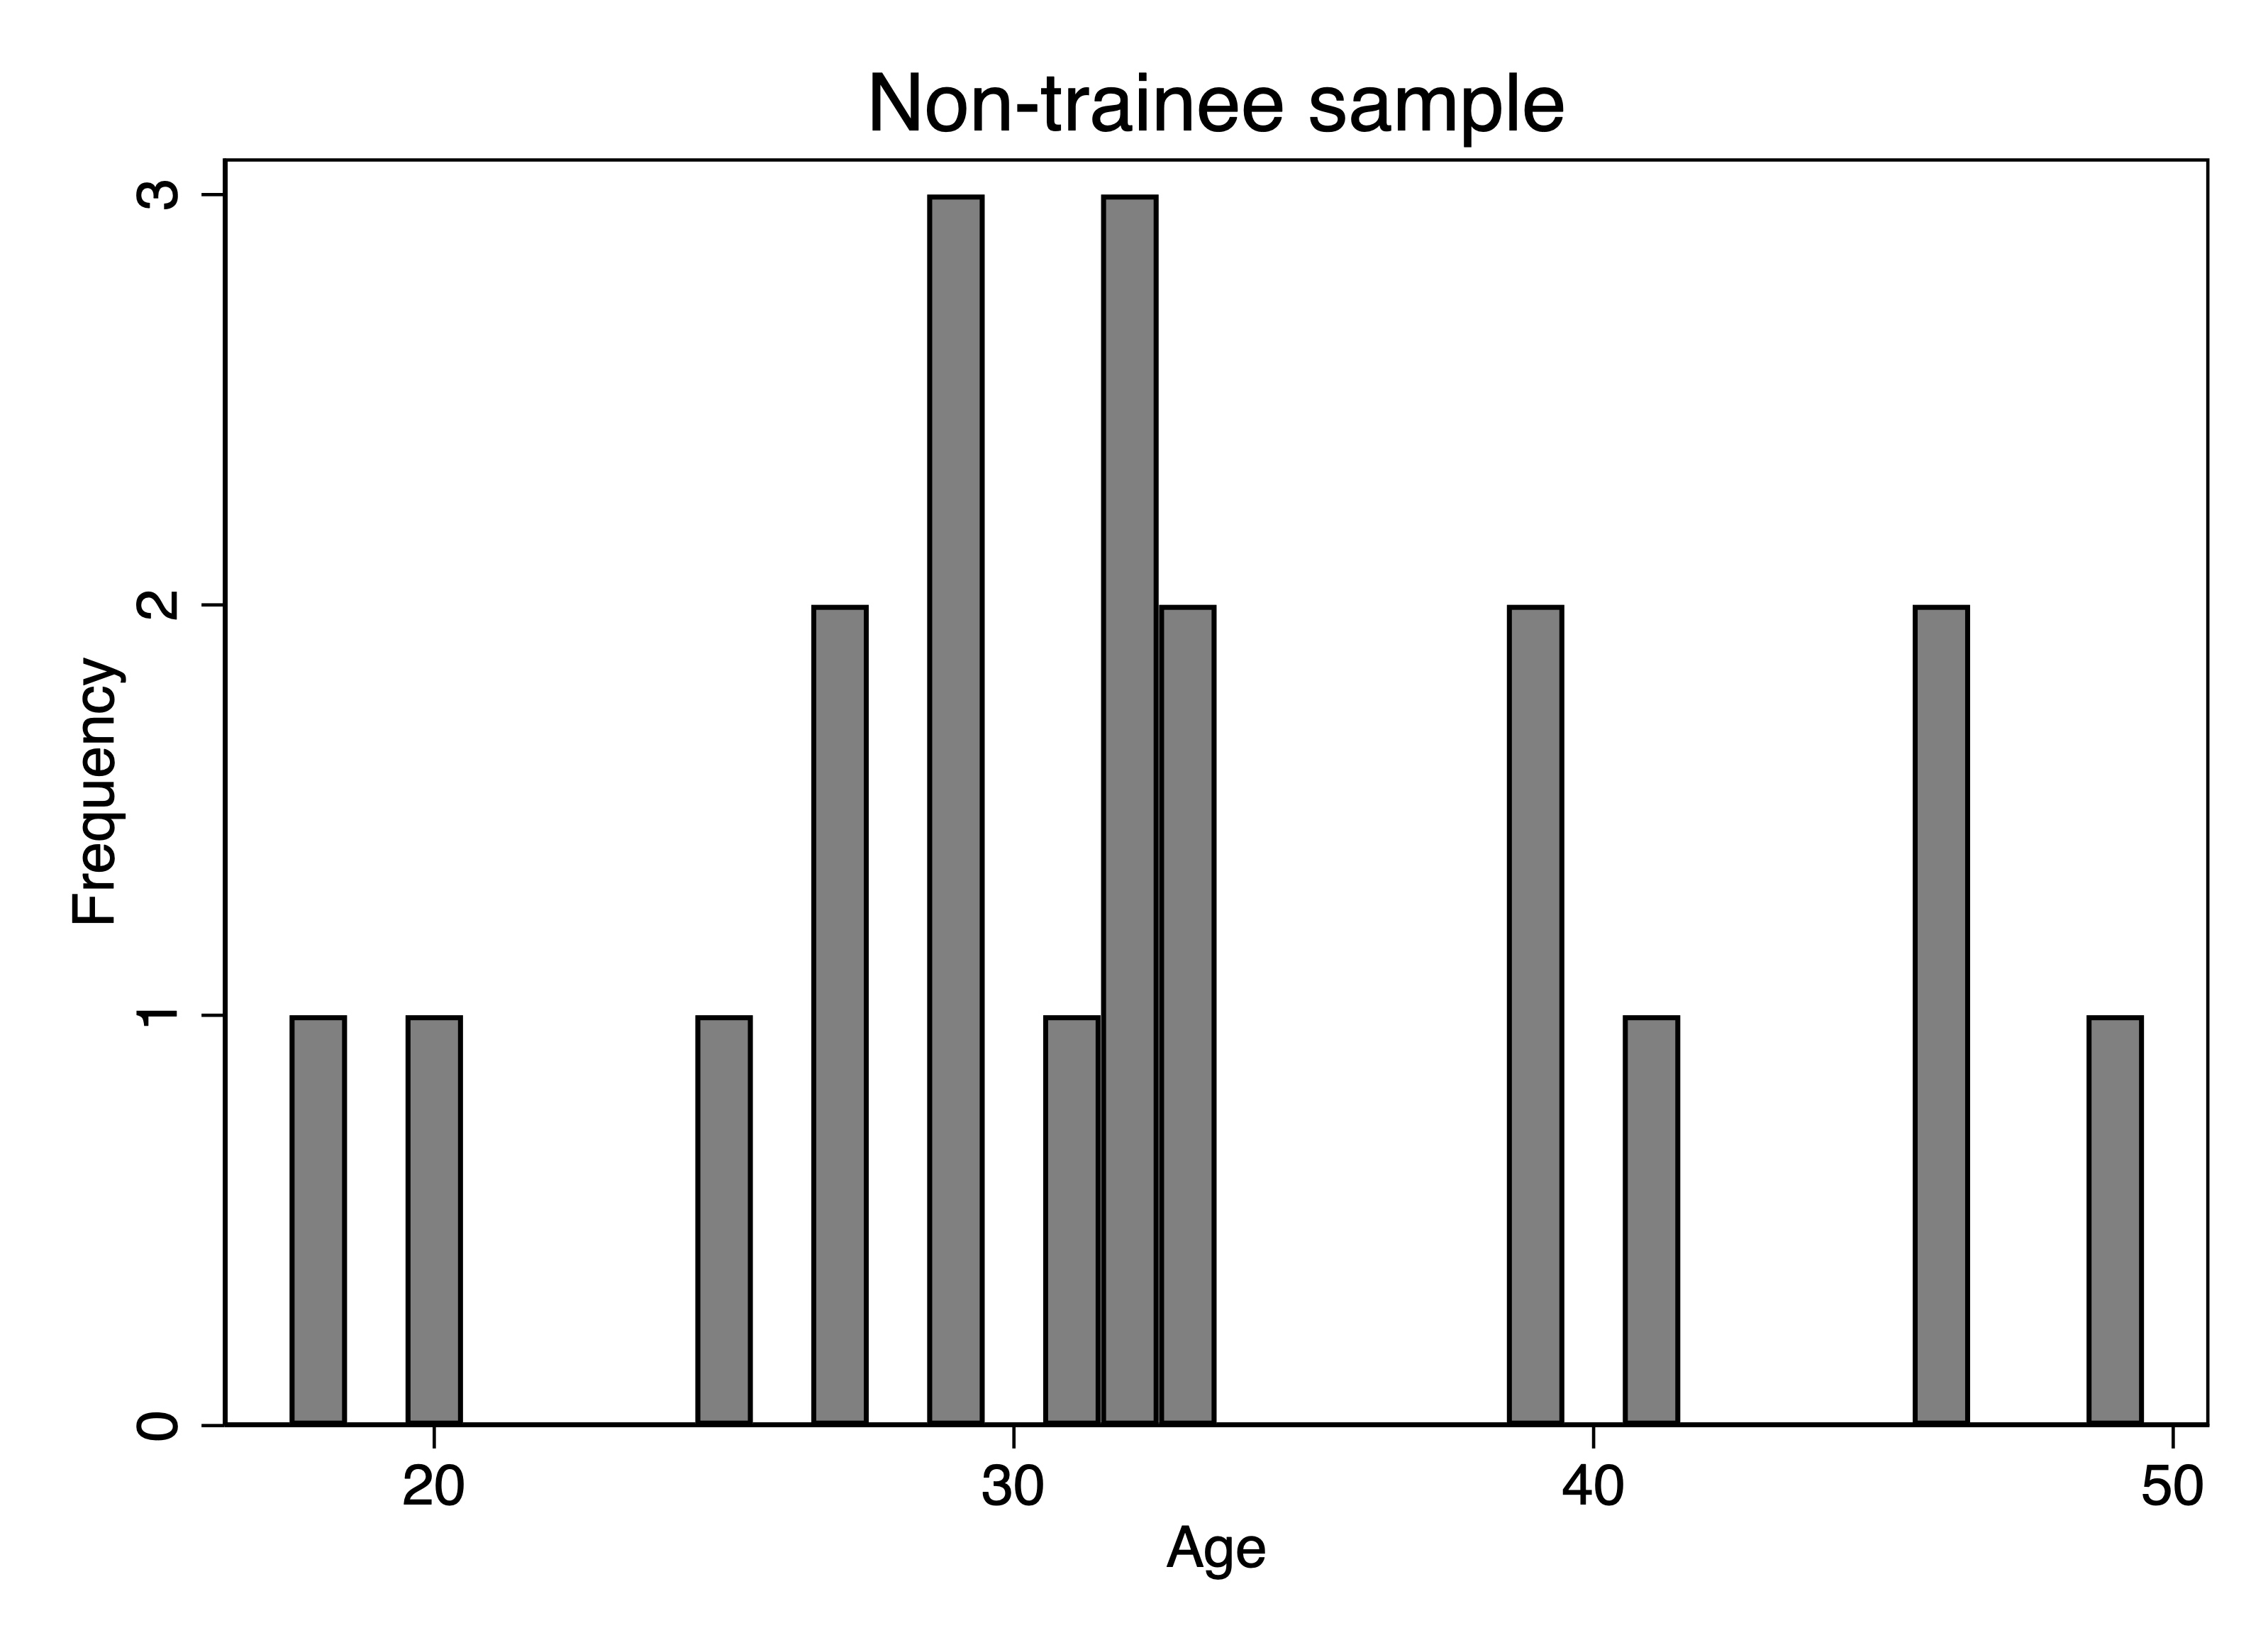
\includegraphics[scale=0.075]{./lecture_includes/nontrainees}
\end{figure}

\end{frame}

\begin{frame}{Exact matching}

\begin{itemize}
\item Exact matching finds a person in the control group whose value of $X_j$ is \emph{exactly} equal to each person in the treatment group $i$
\item Will not work if the conditioning set includes a continuous variable
\item Will also not work if $K$ gets large (curse of dimensionality)
\item But let's see it work now
\end{itemize}

\end{frame}

\begin{frame}{Matching algorithm}

\begin{enumerate}
\item For each unit $i$ in the treatment group with known and quantified confounder $X=x_i$, find all units $j$ in the donor pool for whom $x_i=x_j$. These $j$ units are our $M$ matches and $M$ can be one or it can be greater than one if you want it to be.
\item For each unit $i$, replace its missing potential outcome, $Y^0_i$, with the matched $j$ units' realized outcomes, $\frac{1}{M} \sum {Y}_{j(i)}$, from Step 1. Do this for all $i$ units in the treatment group.
\item For each unit $i$, calculate the difference between realized earnings and matched earnings, $\widehat{\delta}_i=Y_i - \frac{1}{M} \sum {Y}_{j(i)}$.
\item Finally, estimate the sample ATT by averaging over all $i$ differences in earnings from Step 3 as $\frac{1}{N_T} \sum \widehat{\delta}_i$, where $N_T$ is the number of treatment units.
\end{enumerate}

\end{frame}

\begin{frame}{Look at commands}

Let's now look at this using simulated data. Lab is incomplete so this is just illustrative.  

\end{frame}


\begin{frame}{Matched sample}

\begin{table}[htb]\small\index{rolling!3}
\caption{Training example with matched sample using exact matching}
\centering
\begin{tabular}{ccc|ccc}
\toprule
	\multicolumn{3}{c}{\textbf{Trainees}}&
	\multicolumn{3}{c}{\textbf{Matched Sample}}\\
	\multicolumn{1}{c}{Unit}&
	\multicolumn{1}{c}{Age}&
	\multicolumn{1}{c}{Earnings}&
	\multicolumn{1}{c}{Matched Unit}&
	\multicolumn{1}{c}{Age}&
	\multicolumn{1}{c}{Earnings}\\
\midrule
1&	31&	\$26,693&	2&	31&	\$25,052 \\
2&	31&	\$26,691&	2&	31&	\$25,052 \\
3&	18&	\$15,392&	18&	18&	\$15,046 \\
4&	32&	\$27,776&	5&	32&	\$26,045 \\
5&	32&	\$27,779&	5&	32&	\$26,045 \\
6&	25&	\$20,821&	4&	25&	\$19,787 \\
7&	32&	\$27,778&	5&	32&	\$26,045 \\
8&	32&	\$27,780&	5&	32&	\$26,045 \\
9&	20&	\$16,781&	8&	20&	\$16,246 \\
10&	29&	\$24,610&	6&	29&	\$23,178 \\
\midrule
Mean&	28.2&	\$24,210&	Mean&	28.2&	\$22,854 \\
\bottomrule
\end{tabular}
\label{tab:trainee2}
\end{table}

\end{frame}

\begin{frame}{Estimated ATT using Exact Matching}

Estimate the ATT using the sample averages in the original treatment dataset and the \emph{matched} sample

\begin{equation}
ATT = \$24,210 - \$22,854 = \$1,356
\end{equation}

\bigskip

Just remember -- this required conditional independence of $Y^0$ with respect to age. If that's not true, then this is just garbage.

\bigskip

Common support means that exact matching is possible.  So the only way we have selection bias is if conditional independence doesn't hold.

\end{frame}


\begin{frame}{Failed matching when attempting to estimate the ATE}

\begin{table}[htb]\tiny\index{rolling!3}
\caption{Failed matches in the non-trainee comparison group}
\centering
\begin{tabular}{lcc}
\toprule
	\multicolumn{3}{c}{\textbf{Non-Trainees}}\\
	\multicolumn{1}{c}{Unit}&
	\multicolumn{1}{c}{Age}&
	\multicolumn{1}{c}{Earnings}\\
\midrule
1&	27&	\$21,416 \\
3&	33&	\$27,059 \\
6&	39&	\$33,815 \\
7&	36&	\$30,297 \\
8&	33&	\$27,061 \\
11&	27&	\$21,418 \\
13&	41&	\$36,316 \\
14&	41&	\$36,316 \\
15&	43&	\$38,940 \\
17&	49&	\$47,559 \\
19&	27&	\$21,416 \\
20&	46&	\$43,112 \\
\bottomrule
\end{tabular}
\label{tab:trainee3}
\end{table}

\end{frame}

\begin{frame}{Cause of failure}

\begin{itemize}

\item We were able to find ``exact matches'' for the ATT because there were comparison units in the control group with exactly the same value of $X$
\item But we could not find ``exact matches'' for our control group in the treatment group, and therefore could not estimate the ATE (or the ATU)
\item Cause: curse of dimensionality broke common support assumption
\item So what can we do if that happens?  

\end{itemize}

\end{frame}


\subsection{Inexact matching with nearest neighbors}

\begin{frame}{Inexact matching}

\begin{figure}[!t]\centering

\includegraphics[scale=0.75]{./lecture_includes/fraternal_twins}
\end{figure}

\end{frame}


\begin{frame}{To Look Like Someone Else}

\begin{itemize}
\item When we can make synthetic xerox copies of ourselves, that's exact matching
\item But what if we can only make similar copies of ourselves, like fraternal, but not identical, twins? That's nearest neighbor matching -- a form of ``inexact matching'', sort of like fraternal twins
\item Introduces bias bc of inexact matching, but the magnitude of the bias depends on the magnitude of the discrepancy
\item There exists a method to reduce the selection bias (Abadie and Imbens 2011)
\end{itemize}

\end{frame}

\begin{frame}{Nearest Neighbor Matching}
	
	\begin{itemize}
	\item Estimate $\delta_{ATT}$ by \emph{imputing} the missing potential outcome of each treatment unit $i$ using the observed outcome from that outcome's ``nearest'' neighbor $j$ in the control set using $X$ for the matching
		\begin{eqnarray*}
		\delta_{ATT} = \frac{1}{N_T}\sum_{D_i=1} (Y_i - Y_{j(i)})
		\end{eqnarray*}where $Y_{j(i)}$ is the observed outcome of a control unit such that $X_{j(i)}$ is the \textbf{closest} value to $X_i$ among all of the control observations (eg match on $X$)
	\end{itemize}
\end{frame}

\begin{frame}{Matching}
	
	\begin{itemize}
	\item We could also use the average observed outcome over $M$ closest matches:
		\begin{eqnarray*}
		\delta_{ATT} = \frac{1}{N_T}\sum_{D_i=1}\left(Y_i-\left[\frac{1}{M}\sum_{m=1}^MY_{j_m(1)}\right]\right)
		\end{eqnarray*}
	\item Works well when we can find good matches for each treatment group unit, so $M$ is usually defined to be small (i.e., $M=1$ or $M=2$)
	\end{itemize}
\end{frame}

\begin{frame}{Matching}
	
	\begin{itemize}
	\item We can also use matching to estimate $\delta_{ATE}$.  In that case, we match in both directions:
		\begin{enumerate}
		\item If observation $i$ is treated, we impute $Y^0_i$ using the control matches,     $\{Y_{j_1(i)}, \dots, Y_{j_M(i)}\}$
		\item If observation $i$ is control, we impute $Y^1_i$ using the treatment matches, $\{Y_{j_1(i)}, \dots, Y_{j_M(i)}\}$
		\end{enumerate}
	\item The estimator is:$$\widehat{\delta}_{ATE} = \frac{1}{N} \sum_{i=1}^N (2D_i -1) \left[ Y_i - \left( \frac{1}{M} \sum_{m=1}^M Y_{j_m(i)} \right) \right]$$	
	\end{itemize}
	
\end{frame}


\begin{frame}{Matching example with single covariate}
	
	\begin{table}
	\begin{tabular}{c|c|c|c|c}
	\hline
	$i$ & $Y^1_i$ & $Y^0_i$ & $D_i$ & $X_i$ \\
	\hline
	1 & 6 &  \textcolor{red}{?} & 1 & 3 \\
	2 & 1 &  \textcolor{red}{?} & 1 & 1 \\
	3 & 0 &   \textcolor{red}{?} & 1 & 10 \\
	\hline
	4 &  & 0 & 0 & 2 \\
	5 &  & 9 & 0 & 3 \\
	6 &  & 1 & 0 & -2 \\
	7 &  & 1 & 0 & -4 \\
	\hline
	\end{tabular}
	\end{table}
	
	
	\begin{flalign*}
		    \only<1-2>{&\text{Question: What is }\widehat{\delta_{ATT}}=\frac{1}{N_T} \sum_{D_i=1} (Y_i - Y_{j(i)})\text{?}}& \\
		    \only<2-2>{&\text{Match and plug in!}} \\
 	\end{flalign*}

\end{frame}
	
	
\begin{frame}{Matching example with single covariate}
	
	\begin{table}
	\begin{tabular}{c|c|c|c|c}
	\hline
	$i$ & $Y^1_i$ & $Y^0_i$ & $D_I$ & $X_i$ \\
	\hline
	1 & 6 &  \textcolor{blue}{9} & 1 & \textcolor{blue}{3} \\
	2 & 1 &  \textcolor{green}{0} & 1 & \textcolor{green}{1} \\
	3 & 0 &   \textcolor{blue}{9} & 1 & \textcolor{blue}{10} \\
	\hline
	4 &  & \textcolor{green}{0} & 0 & \textcolor{green}{2} \\
	5 &  & \textcolor{blue}{9} & 0 & \textcolor{blue}{3} \\
	6 &  & 1 & 0 & -2 \\
	7 &  & 1 & 0 & -4 \\
	\hline
	\end{tabular}
	\end{table}
	
	
	\begin{flalign*}
		&\text{Question: What is }\widehat{\delta_{ATT}}=\frac{1}{N_T} \sum_{D_i=1} (Y_i - Y_{j(i)})\text{?}& \\
		&\widehat{\delta}_{ATT} = \frac{1}{3} \cdot (6-\textcolor{blue}{9}) + \frac{1}{3} \cdot (1-\textcolor{green}{0}) + \frac{1}{3} \cdot (0-\textcolor{blue}{9}) = -3.7
	\end{flalign*}

\end{frame}


%{
%\setbeamercolor{background canvas}{bg=}
%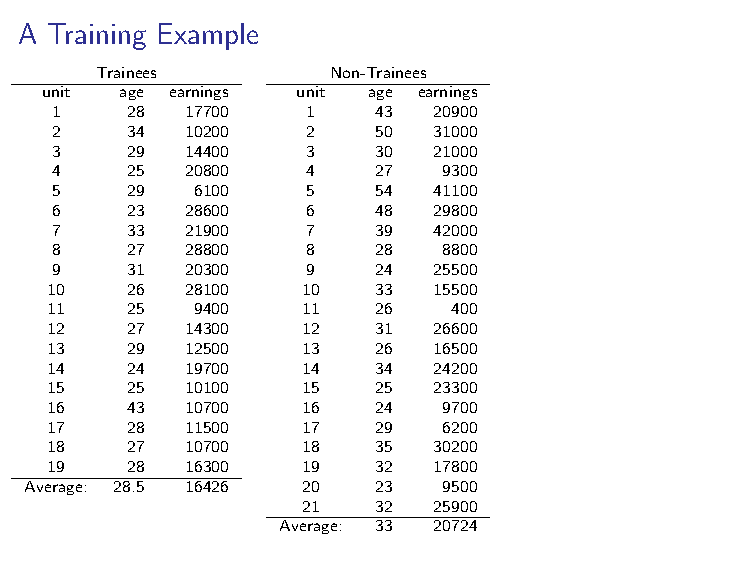
\includepdf[pages=1-last]{./lecture_includes/abadie-matching2.pdf}
%}



\begin{frame}{Measuring the matching discrepancy}

\begin{itemize}
\item What does it mean to be close when I am working with a large number of covariates?
\item What if we had a way of measuring a match in terms of how ``close'' each unit's $X_i$ value was to the matched $X_j$
\item Let's do that and use the square root of the sum of all squared differences in each unit's $X_i - X_{j(i)}$ as a measure of how bad the match is
\item This is called the Euclidean distance
\end{itemize}


\end{frame}

%\begin{frame}{Alternative distance metric: Euclidean distance}
	
% When the vector of matching covariates, $X= \colvec{X_1\\X_2\\\vdots\\X_k}$ has more than one dimension ($k>1$) we will need a new definition of \textbf{distance} to measure ``closeness''.  
%\end{frame}

\begin{frame}{Euclidean distance}
	\begin{block}{Definition: Euclidean distance}
    \vspace*{-2.5mm}
    \begin{eqnarray*}
    ||X_i-X_j|| &=& \sqrt{ (X_i-X_j)'(X_i-X_j) } \\
    &=& \sqrt{ \sum_{n=1}^k (X_{ni} - X_{nj})^2 }
    \end{eqnarray*}
    \vspace*{-2.5mm}
	\end{block}
	
Let's do this together -- sometimes it helps to manually calculate this

\bigskip

\url{https://docs.google.com/spreadsheets/d/1iro1Qzrr1eLDY_LJVzOYvnQZWmxY8JyTcDf6YcdhkwQ/edit?usp=sharing}

	
\end{frame}


\begin{frame}{Inexact matching: Random match 1}

\begin{figure}[!t]\centering
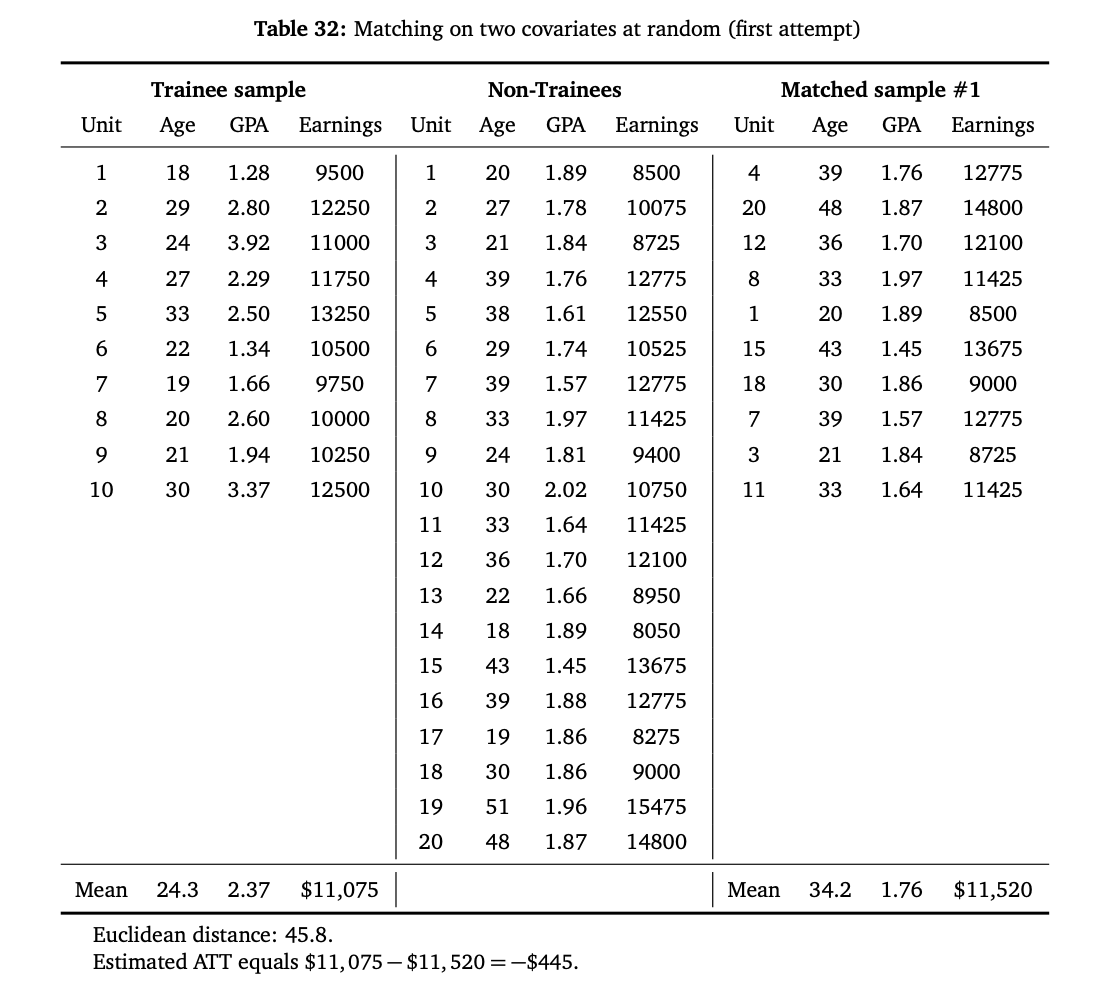
\includegraphics[scale=0.45]{./lecture_includes/inexact_random1}
\end{figure}

\end{frame}


\begin{frame}{Inexact matching: Random match 2}

\begin{figure}[!t]\centering
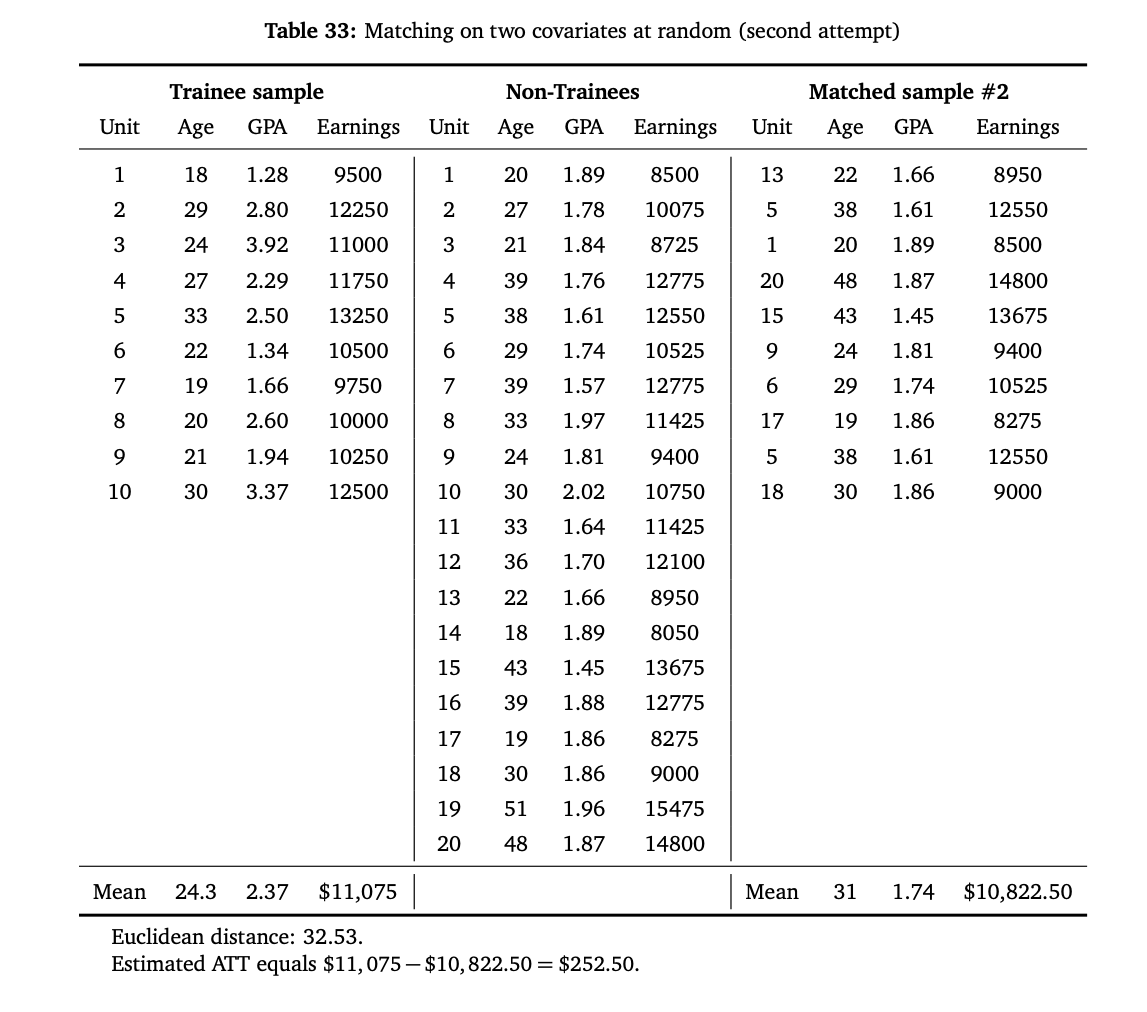
\includegraphics[scale=0.45]{./lecture_includes/inexact_random2}
\end{figure}

\end{frame}


\begin{frame}{Minimizing the Euclidean distance}

\begin{itemize}
\item Abadie and Imbens (2006) show that there exists a matching that minimizes the distance metric
\item Thankfully, this code exists so let's just look at the output
\item But the idea here is that any other match will always have a higher Euclidean distance
\end{itemize}

\end{frame}




\begin{frame}{Inexact matching by minimizing the Euclidean distance}

\begin{figure}[!t]\centering
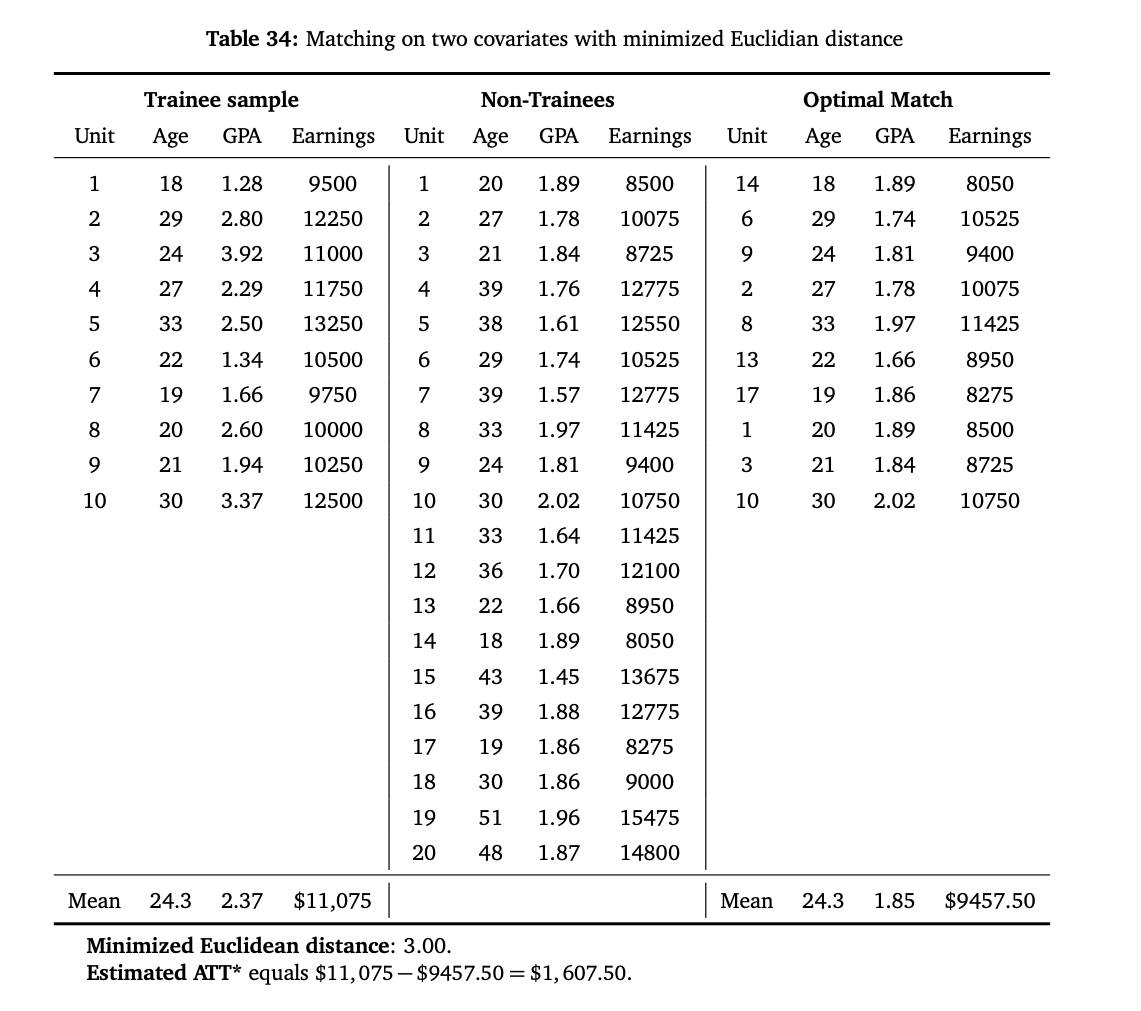
\includegraphics[scale=0.45]{./lecture_includes/inexact_euclidean}
\end{figure}

\end{frame}

\begin{frame}{Other distance metrics}

\begin{itemize}
\item  The Euclidean distance is not invariant to changes in the scale of the $X$'s.  For this reason, alternative distance metrics that \emph{are} invariant to changes in scale are used
\item Normalized Euclidean distance and Mahalanobis distance both try to normalize it so that scale doesn't matter
\item There's a few more, and you may want to explore all of them
\end{itemize}

\end{frame}


\begin{frame}{Normalized Euclidean distance}

	\begin{block}{Definition: Normalized Euclidean distance}
	  A commonly used distance is the normalized Euclidean distance:$$||X_i-X_j|| = \sqrt{ (X_i-X_j)'\widehat{V}^{-1}(X_i - X_j) }$$ where
		$$\widehat{V}^{-1} = \text{diag}(\widehat{\sigma}_1^2, \widehat{\sigma}_2^2, \dots, \widehat{\sigma}_k^2)$$
	\end{block}
\end{frame}

\begin{frame}{Normalized Euclidean distance}
	\begin{itemize}
	\item Notice that the normalized Euclidean distance is equal to:
		\begin{eqnarray*}
		||X_i - X_j|| = \sqrt{\sum_{n=1}^k \frac{(X_{ni} - X_{nj})}{\widehat{\sigma}^2_n}}
		\end{eqnarray*}
	\item Thus, if there are changes in the scale of $X_{ni}$, these changes also affect $\widehat{\sigma}^2_n$, and the normalized Euclidean distance does not change
	\end{itemize}

\end{frame}


\begin{frame}{Mahalanobis distance}
	
	\begin{block}{Definition: Mahalanobis distance}
	The Mahalanobis distance is the scale-invariant distance metric:
		\begin{eqnarray*}
		||X_i-X_j|| = \sqrt{ (X_i-X_j)'\widehat{\Sigma}_X^{-1}(X_i - X_j) }
		\end{eqnarray*}
	where $\widehat{\Sigma}_X$ is the sample variance-covariance matrix of $X$.
	\end{block}


\end{frame}


\begin{frame}{Arbitrary weights}
	
	Or, you could just create your own arbitrary weights
		\begin{eqnarray*}
		||X_i-X_j|| = \sqrt{ \sum_{n=1}^k \omega_n \cdot (X_{ni} - X_{nj})^2}
		\end{eqnarray*}(with all $\omega_n\geq{0}$) so that we assign large $\omega_n$'s to those covariates that we want to match particularly well.

\end{frame}

\begin{frame}{Matching and the Curse of Dimensionality}
	
\begin{itemize}
\item The larger the dimensions of the conditioning set, even if they are needed for identification, the less likely common support holds
\item This problem is caused by the finite dataset, and it introduces selection bias
\item Abadie and Imbens (2011) derived a solution called bias correction matching
\end{itemize}

\end{frame}


\begin{frame}{Deriving the matching bias}
	
  \vspace{-5mm}
  $$
		\widehat{\delta}_{ATT} = \frac{1}{N_T} \sum_{D_i=1} (Y_i - Y_{j(i)}),
  $$
  where each $i$ and $j(i)$ units are matched, $X_i \approx X_{j(i)}$ and $D_{j(i)}=0$. 
	 
  \bigskip
  Define potential outcomes and switching eq.
		\begin{eqnarray*}
      \mu^0(x) &=& E[Y | X=x,D=0] = E[Y^0 | X=x],\\
      \mu^1(x) &=& E[Y | X=x,D=1] = E[Y^1 | X=x],\\
      Y_i &=& \mu^{D_i}(X_i) + \varepsilon_i
		\end{eqnarray*}
\end{frame}

\begin{frame}{Deriving the matching bias}
  Substitute and distribute terms
  \begin{eqnarray*}
    \widehat{\delta}_{ATT} &=& \frac{1}{N_T} \sum_{D_i=1} (Y_i - Y_{j(i)}) \\
    &=& \frac{1}{N_T} \sum_{D_i=1} \left[ (\mu^1(X_i) + \varepsilon_i) - (\mu^0(X_{j(i)}) + \varepsilon_{j(i)}) \right] \\
    &=&  \frac{1}{N_T} \sum_{D_i=1} (\mu^1(X_i) - \mu^0(X_{j(i)})) + \frac{1}{N_T} \sum_{D_i=1}(\varepsilon_i - \varepsilon_{j(i)})
  \end{eqnarray*}
\end{frame}
		

\begin{frame}{Deriving the matching bias}
	
Difference between sample estimate and population parameter is:
		\begin{eqnarray*}
		\widehat{\delta}_{ATT} - \delta_{ATT} &=& \frac{1}{N_T} \sum_{D_i=1} \left( \mu^1(X_i) - \mu^0(X_{j(i)}) - \delta_{ATT}\right) \\
		&+& \frac{1}{N_T} \sum_{D_i=1} (\varepsilon_i - \varepsilon_{j(i)})
		\end{eqnarray*}
Algebraic manipulation and simplification:
		\begin{eqnarray*}
		\widehat{\delta}_{ATT} - \delta_{ATT} &=& \frac{1}{N_T} \sum_{D_i=1} \left( \mu^1(X_i) - \mu^0(X_i) - \delta_{ATT}\right) \\
		&+& \frac{1}{N_T} \sum_{D_i=1} (\varepsilon_i - \varepsilon_{j(i)}) \\
		&+& \frac{1}{N_T} \sum_{D_i=1} \left( \mu^0(X_i) - \mu^0(X_{j(i)}) \right).
		\end{eqnarray*}
\end{frame}


\begin{frame}{Deriving the matching bias}
	
Note $\widehat{\delta}_{ATT} - \delta_{ATT} \to 0$ as $N \to \infty$.
\pause However, 
$$E[ \sqrt{\frac{1}{N}} (\widehat{\delta}_{ATT} - \delta_{ATT})] = E[ \sqrt{\frac{1}{N}} ( \mu^0(X_i) - \mu^0(X_{j(i)}) ) | D=1].$$ 
\pause
Now consider the implications if $k$ is large:
\pause	\begin{itemize}
	\item The difference between $X_i$ and $X_{j(i)}$ converges to zero very slowly 
\pause	\item The difference $\mu^0(X_i) - \mu^0(X_{j(i)})$ converges to zero very slowly \pause
	\item $E[ \sqrt{\frac{1}{N}} (\mu^0(X_i) - \mu^0(X_{j(i)})) | D=1]$ may not converge to zero and an be very large! 
\pause	\item $E[ \sqrt{\frac{1}{N}} (\widehat{\delta}_{ATT} - \delta_{ATT})]$ may not converge to zero because the bias of the matching discrepancy is dominating the matching estimator! \pause
	\end{itemize}
 Bias is often an issue when we match in many dimensions
\end{frame}

\begin{frame}{Solutions to matching bias problem}
	
The bias of the matching estimator is caused by large matching discrepancies $||X_i - X_{j(i)}||$ which is virtually guaranteed by the curse of dimensionality.  However:
	\begin{enumerate}
	\item But the matching discrepancies are observed. We can always check in the data how well we're matching the covariates.

	\item For $\widehat{\delta}_{ATT}$ we can sometimes make the matching discrepancies small by using a large reservoir of untreated units to select the matches (that is, by making $N_C$ large).

  \item If the matching discrepancies are large, so we are worried about potential biases, we can apply bias correction techniques

	\end{enumerate}
\end{frame}


\begin{frame}{Matching with bias correction}
	
	\begin{itemize}
	\item Each treated observation contributes$$\mu^0(X_i) - \mu^0(X_{j(i)})$$to the bias.
	\item Bias-corrected (BC) matching:
		\begin{eqnarray*}
		\widehat{\delta}_{ATT}^{BC} = \frac{1}{N_T} \sum_{D_i=1} \left[ (Y_i - Y_{j(i)}) - ( \widehat{\mu^0}(X_i) - \widehat{\mu^0}(X_{j(i)}) ) \right]
		\end{eqnarray*}where $\widehat{\mu^0}(X)$ is an estimate of $E[Y|X=x,D=0]$.  For example using OLS.  
	\item Under some conditions, the bias correction eliminates the bias of the matching estimator without affecting the variance.
	\end{itemize}
\end{frame}


\begin{frame}{Steps}

\begin{enumerate}
\item[1.  ]Regress $Y$ on $X$ with OLS except only use the control sample:
\begin{equation}
Y_j = \alpha + \beta X_j + \varepsilon_j \nonumber
\end{equation}where $j$ are the units for which $D_j=0$.  
\end{enumerate}

\end{frame}

\begin{frame}{Steps}

\begin{enumerate}
\item[2. ] Use the fitted values $\widehat{\alpha}$ and $\widehat{\beta}$ to predict $\widehat{\mu}^0(X)$ for both the $i$ and the matched $j(i)$ units:
\begin{eqnarray}
\widehat{\mu}^0_i &=& \widehat{\alpha} + \widehat{\beta} X_i \nonumber \\
\widehat{\mu}^0_{j(i)} &=& \widehat{\alpha} + \widehat{\beta} X_{j(i)} \nonumber
\end{eqnarray}
\end{enumerate}

\end{frame}


\begin{frame}{Steps}

\begin{enumerate}
\item[3. ] Subtract $ \widehat{\mu}_i^0(X_i) - \widehat{\mu}_{j(i)}^0(X_{j(i)})$, our estimate of the selection bias caused by matching discrepancies, from the sample estimate of the $ATT$: $$\widehat{\delta}_{ATT}^{BC} = \dfrac{1}{N_T} \sum_{D_i=1} \bigg [ (Y_i - Y_{j(i)}) - \Big(\widehat{\mu}^0(X_i) - \widehat{\mu}^0(X_{j(i)})\Big) \bigg ]$$
\end{enumerate}

\end{frame}


\begin{frame}{Steps}

\begin{enumerate}
\item[4. ] Estimate Abadie-Imbens robust standard error (Abadie and Imbens 2006; 2008; 2011)
\end{enumerate}

\end{frame}



\begin{frame}[plain,shrink=0]
	\begin{center}
	\textbf{Bias adjustment in matched data}
	\end{center}
	
	\begin{table}
	\begin{tabular}{c|c|c|c|c}
	\hline
	\multicolumn{1}{c}{}&
	\multicolumn{2}{c}{Potential Outcome}&
	\multicolumn{1}{c}{}&
	\multicolumn{1}{c}{}\\
	\multicolumn{1}{c}{unit} &
	\multicolumn{1}{c}{under Treatment}&
	\multicolumn{1}{c}{under Control}&
	\multicolumn{1}{c}{}&
	\multicolumn{1}{c}{}\\
	\hline
	$i$ & $Y^1_i$ & $Y^0_i$ & $D_i$ & $X_i$ \\
	\hline
	1 & \textcolor{blue}{10} &  \textcolor{blue}{8} & 1 & \textcolor{blue}{3} \\
	2 & 4 &  			 1 &				 1 & 1 \\
	3 & \textcolor{green}{10} &   \textcolor{green}{9} & 1 & \textcolor{green}{10} \\
	\hline
	4 &  & \textcolor{blue}{8} & 0 & \textcolor{green}{4} \\
	5 &  & 			 1 & 0 &  				0 \\
	6 &  & \textcolor{green}{9} & 0 & \textcolor{green}{8} \\
	\hline
	\end{tabular}
	\end{table}
	
	
	\begin{flalign*}
		\only<1-3>{&\widehat{\delta}_{ATT} = \frac{10-8}{3} + \frac{4-1}{3}  + \frac{10-9}{3}  = 2&} \\
		\only<2-3>{&\text{For the bias correction, estimate }\widehat{\mu^0}(X) = \widehat{\beta_0} + \widehat{\beta_1}X = 2+X}\\
		\only<3-3>{&\widehat{\delta}_{ATT} = \frac{ (10-8) - ( \widehat{\mu^0}(3) - \widehat{\mu^0}(4)) }{3}  + \frac{ (4-1)  -( \widehat{\mu^0}(1) - \widehat{\mu^0}(0)) }{3}  \\
		&+ \frac{ (10-9)  - ( \widehat{\mu^0}(10) - \widehat{\mu^0}(8))}{3} = 1.33}
	\end{flalign*}

\end{frame}


\begin{frame}{Matching bias: Implications for practice}
	
\emph{Matching} bias arises because of the effect of large matching discrepancies on $\mu^0(X_i) - \mu^0(X_{j(i)})$ due to a lack of common support. To minimize matching discrepancies:
	\begin{enumerate}
	\item Use a small $M$ (e.g., $M=1$). Larger values of $M$ produce large matching discrepancies.
	\item Use matching with replacement.  Because matching with replacement can use untreated units as a match more than once, matching with replacement produces smaller matching discrepancies than matching without replacement.
	\item Try to match covariates with a large effect on $\mu^0(\cdot)$ particularly well.
	\end{enumerate}
\end{frame}

\begin{frame}{Large sample distribution for matching estimators}
	
	\begin{itemize}
	\item Cannot use the bootstrap, so Abadie and Imbens derived the variance (Abadie and Imbens 2008)
	\item Matching estimators have a Normal distribution in large samples (provided the bias is small):
		\begin{eqnarray*}
		\sqrt{N_T} (\widehat{\delta}_{ATT} - \delta_{ATT}) \xrightarrow{d} N(0,\sigma^2_{ATT})
		\end{eqnarray*}
	\item For matching without replacement, the ``usual'' variance estimator:
		\begin{eqnarray*}
		\widehat{\sigma}^2_{ATT} = \frac{1}{N_T} \sum_{D_i=1} \left( Y_i - \frac{1}{M} \sum_{m=1}^M Y_{j_m(i)} - \widehat{\delta}_{ATT} \right)^2,
		\end{eqnarray*}is valid.
	\end{itemize}
\end{frame}

\begin{frame}{Large sample distribution for matching estimators}
	
	\begin{itemize}
	\item For matching with replacement:
		\begin{eqnarray*}
		\widehat{\sigma}^2_{ATT} &=& \frac{1}{N_T} \sum_{D_i=1} \left( Y_i - \frac{1}{M} \sum_{m=1}^M Y_{j_m(i)} - \widehat{\delta}_{ATT} \right)^2 \\
		&+& \frac{1}{N_T} \sum_{D_i=0} \left( \frac{K_i(K_i-1)}{M^2} \right) \widehat{var}(\varepsilon | X_i,D_i=0)
		\end{eqnarray*}where $K_i$ is the number of times observation $i$ is used as a match.
	\item $\widehat{var}(Y_i | X_i,D_i=0)$ can be estimated also by matching.  For example, take two observations with $D_i=D_j=0$ and $X_i \approx X_j$, then
		\begin{eqnarray*}
		\widehat{var}(Y_i | X_i,D_i=0) = \frac{(Y_i-Y_j)^2}{2}
		\end{eqnarray*}is an unbiased estimator of $\widehat{var}(\varepsilon_i | X_i,D_i=0))$
	\end{itemize}
\end{frame}

\begin{frame}{Final note about bias adjustment}

\begin{itemize}
\item Identifying assumptions with selection on observables are:
	\begin{enumerate}
	\item Potential outcomes are distributed independent of treatment status (``conditional independence'')
	\item Common support
	\end{enumerate}
\item Matching discrepancies are due to violations of second assumption caused by curse of dimensionality -- not the first
\item Matching bias adjustments \textbf{do not} recover ATE or ATT if conditional independence fails as that implies omitting a possibly very important and influential confounder
\end{itemize}

\end{frame}

\subsection{Regressions}

\begin{frame}{Frisch-Waugh-Lovell theorem}

	\begin{itemize}
	\item FWL theorem concerns multiple linear regression.
	\item Can we estimate the causal effect of family size on labor supply by regressing labor supply (\texttt{Y}) on family size (\texttt{X})?
		\begin{align*}
		Y_i = \beta_0 + \beta_1 X_i + u_i&\\
		\end{align*}
	\item If family size is random, then number of kids is uncorrelated with the unobserved error term, which means we can interpret $\widehat{\beta_1}$ as the causal effect.
	\item But how do we interpret $\widehat{\beta_1}$ if \texttt{numkids} is non-random?  
	\end{itemize}
\end{frame}


\begin{frame}{FWL Theorem}
	
	\begin{itemize}
	\item Assume that family size is random once we condition on race, age, marital status and employment.  Then the model is:
		\begin{eqnarray*}
Y_i &=& \beta_0 + \beta_1 X_i + \gamma_1 \texttt{White}_i + \gamma_2 \texttt{Married}_i \\
		& & + \gamma_3 \texttt{Age}_i + \gamma_4 \texttt{Employed}_i + u_i
		\end{eqnarray*}
	\item If we want to estimate average causal effect of family size on labor supply, we will need two things: 
		\begin{enumerate}
		\item a data set with all $6$ variables; 
		\item Number of kids ($X_i$) must be randomly assigned conditional on the other $4$ variables
		\end{enumerate}
	\item How do we interpret $\widehat{\beta_1}$ with the additional controls?
	\end{itemize}
	
\end{frame}

\begin{frame}{FWL Theorem}

\begin{itemize}
\item Frisch-Waugh-Lovell theorem (FWL) is about interpretation of a regression coefficient, like $\widehat{\beta}_1$ when there are covariates
\item Angrist and Pischke (2009) call this the ``regression anatomy theorem'', as does Filoso (2013)
\item Allows you to also convert a multivariate regression into a univariate regression which can help with interpretation and visualization
\item It says that $\widehat{\beta_1}$ is simply a scaled covariance with the $\tilde{x_1}$ residual used instead of the actual data $x$
\item Filoso (2013) has an excellent simplification of the historical more complex proof
\end{itemize}

\end{frame}

		

\begin{frame}{FWL Theorem}

	\begin{block}{FWL Theorem }
	Assume your main multiple regression model of interest:$$y_i=\beta_0 + \beta_1x_{1i} + \dots + \beta_kx_{ki} + \dots + \beta_Kx_{Ki} + e_i$$ and an auxiliary regression in which the variable $x_{1i}$ is regressed on all the remaining independent variables$$x_{1i} = \gamma_0 + \gamma_{k-1}x_{k-1 i}+\gamma_{k+1}x_{k+1 i} + \dots + \gamma_Kx_{Ki}+f_i$$and $\tilde{x}_{1i} = x_{1i} - \widehat{x}_{1i}$ being the residual from the auxiliary regression. The parameter $\beta_1$ can be rewritten as:$$\beta_1=\frac{Cov(y_i,\tilde{x}_{1i})}{Var(\tilde{x}_{1i})}$$

	\end{block}

\end{frame}


\begin{frame}[plain, shrink=20]

\bigskip

	\begin{block}{FWL Proof  (Proof by Filoso 2013)}
	To prove the theorem, note $E[\tilde{x}_{ki}]=E[x_{ki}]-E[\widehat{x}_{ki}]=E[f_i]$, and plug $y_i$ and residual $\tilde{x}_{ki}$ from $x_{ki}$ auxiliary regression into the covariance $cov(y_i, \tilde{x}_{ki})$
	\begin{eqnarray*}
	\beta_k &=& \frac{ cov(y_i, \tilde{x}_{ki})}{var(\tilde{x}_{ki})} \\
			 &=& \frac{ cov(\beta_0 + \beta_1x_{1i} + \dots + \beta_kx_{ki} + \dots + \beta_Kx_{Ki} + e_i, \tilde{x}_{ki})}{var(\tilde{x}_{ki})} \\
			&=& \frac{ cov(\beta_0 + \beta_1x_{1i} + \dots + \beta_kx_{ki} + \dots + \beta_Kx_{Ki} + e_i,f_i)}{var(f_i)}
	\end{eqnarray*}
	\begin{enumerate}
	\item Since by construction $E[f_i]=0$, it follows that the term $\beta_0E[f_i]=0$.
	\item Since $f_i$ is a linear combination of all the independent variables with the exception of $x_{ki}$, it must be that$$\beta_1E[f_ix_{1i}] = \dots = \beta_{k-1}E[f_ix_{k-1 i}] = \beta_{k+1}E[f_ix_{k+1 i}] = \dots = \beta_KE[f_ix_{KI}] = 0$$
	\end{enumerate}
	\end{block}
\end{frame}


\begin{frame}[plain, shrink=20]

	\begin{block}{FWL Proof  (Proof by Filoso 2013)}
		\begin{enumerate}\addtocounter{enumi}{2}
		\item Consider now the term $E[e_if_i]$.  This can be written as:
			\begin{eqnarray*}
			E[e_if_i] &=& E[e_if_i] \\
			&=& E[e_i\tilde{x}_{ki}] \\
			&=& E[e_i(x_{ki} - \widehat{x}_{ki})] \\
			&=& E[e_ix_{ki}] - E[e_i\tilde{x}_{ki}]
			\end{eqnarray*}Since $e_i$ is uncorrelated with any independent variable, it is also uncorrelated with $x_{ki}$: accordingly, we have $E[e_ix_{ki}]=0$. With regard to the second term of the subtraction, substituting the predicted value from the $x_{ki}$ auxiliary regression, we get$$E[e_i\tilde{x}_{ki}] = E[e_i(\widehat{\gamma_0} + \widehat{\gamma_1}x_{1i} + \dots + \widehat{\gamma}_{k-1}x_{k-1}i+\widehat{\gamma}_{k+1}x_{k+1 i} + \dots + \widehat{\gamma}_Kx_{Ki})]$$Once again, since $e_i$ is uncorrelated with any independent variable, the expected value of the terms is equal to zero.  Then, it follows $E[e_if_i]=0$.
		
		\end{enumerate}
	\end{block}

\end{frame}

\begin{frame}[plain, shrink=25]

	\begin{block}{FWL Proof  (Proof by Filoso 2013)}
		\begin{enumerate}\addtocounter{enumi}{3}
		\item The only remaining term is $E[\beta_kx_{ki}f_i]$ which equals $E[\beta_kx_{ki}\tilde{x}_{ki}]$ since $f_i=\tilde{x}_{ki}$. The term $x_{ki}$ can be substituted using a rewriting of the auxiliary regression model, $x_{ki}$, such that$$x_{ki} = E[x_{ki} | X_{-k}] + \tilde{x}_{ki}$$This gives
			\begin{eqnarray*}
			E[\beta_kx_{ki}\tilde{x}_{ki}] &=& E[\beta_kE[\tilde{x}_{ki}(E[x_{ki}|X_{-k}]+\tilde{x}_{ki})]] \\
			&=& \beta_kE[\tilde{x}_{ki}(E[x_{ki}|X_{-k}]+\tilde{x}_{ki})] \\
			&=&\beta_k\{E[\tilde{x}^2_{ki}] + E[(E[x_{ki}|X_{-k}]\tilde{x}_{ki})]\} \\
			&=& \beta_k var(\tilde{x}_{ki})
			\end{eqnarray*}which follows directly from the orthogonoality between $E[x_{ki} | X_{-k}]$ and $\tilde{x}_{ki}$. From previous derivations we finally get$$cov(y_i,\tilde{x}_{ki}) = \beta_kvar(\tilde{x}_{ki})$$which completes the proof. \qedhere
		\end{enumerate}
	\end{block}

\end{frame}

\begin{frame}{FWL}

\begin{itemize}
\item Let's review the FWL ``partialing out'' interpretation of OLS estimated $\widehat{\beta_1}$ in code
\item We will use the fwl.so at /Labs/Matching for this
\end{itemize}

\end{frame}



	

\begin{frame}{Linear regression}

\begin{itemize}
\item Under constant treatment effects, then given exogeneity of the error with respect to covariates, OLS is unbiased estimator of the constant causal effect
\item It is also best of all linear unbiased estimators (BLUE)
\item But as Imbens and Rubin (2015) note here, complex functional forms and heterogeneous treatment effects create some challenges
\end{itemize}

\end{frame}


\begin{frame}{What about OLS?  (Imbens and Rubin 2015)}

	\begin{quote} 
	``In many empirical studies in social sciences, causal effects are estimated through linear regression, where, typically it is implicitly assumed that in the super-population, $$E[Y_i^D | X_i] = \alpha + \delta_{sp} \cdot D + X_i \beta$$ for some values of the three unknown parameters, $\alpha$, $\delta_{sp}$ and $\beta$ where $\delta_{sp} = E_{sp} [ Y_i^1 - Y_i^0]$.''
	\end{quote}
	
\end{frame}

\begin{frame}{What about OLS?  (Imbens and Rubin 2015)}

\begin{quote}
``Defining $\varepsilon_i = Y_i - \delta_{sp} \cdot D_i - X_i \beta$ so that we can write $$Y_i = \alpha + \delta_{sp} \cdot D_i + X_i \beta  + \varepsilon_i$$ it is then assumed that $$\varepsilon_i \independent D_i, X_i$$This assumption is often referred to as \textbf{exogeneity} of the treatment (and the pre-treatment variables) in the econometrics literature.''

\end{quote}

\end{frame}

\begin{frame}{What about OLS?  (Imbens and Rubin 2015)}

\begin{quote}
``The regression function is interpreted as a causal relation, in our sense of the term ``causal'', namely that if we manipulate the treatment $D_i$, then tht outcome would change in expectation by an amount $\delta_{sp}$.  Hence in the potential outcomes formulation, we have 
\begin{eqnarray*}
Y_i^0 &=& \alpha + X_i \beta + \varepsilon_i \\ 
Y_i^1 &=& Y_i^0 + \delta_{sp}
\end{eqnarray*} 

\end{quote}
	
\end{frame}

\begin{frame}{What about OLS?  (Imbens and Rubin 2015)}

\begin{quote}
``Then, because $\varepsilon_i$ is a function of $Y^0_i$ and $X_i$ given the parameters, $$Pr(D_i=1 | Y_i^0, Y_i^1 X_i ) = Pr(D_i | \varepsilon_i, X_i),$$ and by exogeneity of the treatment indicator, we have $$Pr(D_i|\varepsilon_i, X_i) = Pr(D_i | X_i)$$ and thus [conditional independence] holds.'' 
\end{quote}

\end{frame}

\begin{frame}{What about OLS?  (Imbens and Rubin 2015)}

\begin{quote}
\textbf{``However, the exogeneity assumption combines [conditional independence] with functional form and constant treatment effect assumptions that are quite strong, and arguably unnecessary.''}
\end{quote}

\end{frame}

\begin{frame}{Illustration}

\begin{enumerate}

\item Contrast matching with exact matching, constant treatment effects and additive treatment effects and OLS using \texttt{constant\_te.do}
\item Contrast inexact matching, heterogeneous treatment effects, and nonlinearities with small selection bias and OLS using \texttt{training_inexact.do}
\item Contrast matching with inexact matching, heterogeneous treatment effects, and nonlinearities and OLS with significant common support problems and bias adjustment using \texttt{matching.do}
\end{itemize}

\end{enumerate}


		  
\subsection{Propensity scores}

\begin{frame}{Avoiding dimensionality problems}
	
	\begin{itemize}
	\item Curse of dimensionality makes matching on $K$ covariates challenging but earlier work before nearest neighbor covariate matching existed
	\item Rubin (1977) and Rosenbaum and Rubin (1983) developed the propensity score method which reduced $K$ covariates used for adjusting into a single scalar
	\item Insofar as treatment is random conditional on $K$ covariates, then one can use the propensity score to adjust for confounders
	\item Variety of ways to incorporate the propensity score, but first we describe the propensity score as a dimension reduction method 
	\end{itemize}
	
\end{frame}






\begin{frame}{Basic idea behind propensity scores}
	
	\begin{itemize}
	\item Earlier we matched on $X$'s to compare units ``near'' one another based on some distance but matching discrepancies and sparseness created problems
	\item Propensity scores summarize covariate information about treatment selection into a single number bounded between 0 and 1 (i.e., a probability)
	\item Rather than compare units with similar values of $X$, we compare units with similar \textbf{estimated conditional probabilities of treatment}
	\item Important theorem shows that once we adjust comparisons using the propensity score, we do not need to adjust for $X$
	\end{itemize}
\end{frame}



\begin{frame}{Formal Definition}
	
	\begin{block}{Definition of Propensity score}
	A propensity score is a number bounded between 0 and 1 measuring the probability of treatment assignment conditional on a vector of confounding variables: $p(X)=Pr(D=1 | X)$
	\end{block}

\end{frame}

\begin{frame}{Assumptions}

	Two sufficient and necessary identification assumptions:
	\begin{enumerate}
	\item $(Y^0,Y^1) \independent{D}|X$ (conditional independence assumption, CIA)
	\item $0<Pr(D=1|X)<1$ (common support)
	\end{enumerate}
	
	With both, we can incorporate the propensity score into comparisons of treated and untreated units and obtain unbiased and consistent estimates of the ATE

\end{frame}


\begin{frame}{Propensity score methods}
	
Covariate adjustment using the propensity score is a three step process	
		\begin{enumerate}
		\item Estimate the propensity score using logit/probit
		\item Estimate a particular average treatment effect (e.g., ATE, ATT) incorporating the estimated propensity score (e.g., stratification, imputation, regression, or inverse probability weighting)
		\item Estimate standard errors
		\end{enumerate}

Between steps 1 and 2 are various design-like diagnostic steps such as examining common support	using histograms, trimming, etc.

\end{frame}

\begin{frame}{Step 1: Estimating the propensity score}

		\begin{itemize}
		\item Estimate the conditional probability of treatment using probit or logit model$$Pr(D_i=1|X_i) = F(\beta X_i)$$
		\item Use the estimated coefficients to calculate the propensity score for each unit $i$$$\widehat{\rho}_i(X_i) = \widehat{\beta} X_i$$
		\item Note that each unit $i$ now has a predicted probability of treatment given the values of their covariates relative to everyone else's 
		\item Frequentist probability -- you've basically just obtained the likelihood someone who ``looks like you'' would be treated (regardless of whether you were in fact treated)
		\end{itemize}
\end{frame}

\begin{frame}{Identification}
	
	\begin{itemize}
	\item Write down the definition of the ATE conditional on $X_i$
		\begin{eqnarray*}
		E[\delta_i(X_i) ]&=& E[Y^1_i - Y^0_i | X_i=x] \\
		&=&E[Y^1_i | X_i=x] - E[Y^0_i | X_i=x]
		\end{eqnarray*}
	\item Given conditional independence, we can substitute average values of $Y$ for potential outcomes using the switching equation: $$E[Y_i | D_i =1, X_i=x]=E[Y_i^1 | D_i=1, X_i=x]$$ and similar for other term $Y^0$
	\item We need common support (assumption 2) so that both terms can be estimated
	\end{itemize}
\end{frame}		


\begin{frame}{Propensity score theorem}
	
	\begin{block}{Propensity score theorem}
	If $(Y^1,Y^0)\independent{D}|X$ (CIA), then $(Y^1,Y^0)\independent{D} | \rho(X)$ where $\rho(X)=Pr(D=1|X)$, the propensity score
	\end{block}
	
	\begin{itemize}
	\item Conditioning on the propensity score is enough to have independence between $D$ and $(Y^1,Y^0)$ (Rosenbaum and Rubin 1983)
	 \item Valuable theorem because of dimension reduction and convergence rate issues which can introduce biases
	\end{itemize}
\end{frame}

\begin{frame}{Propensity score theorem}
	
	\begin{itemize}
	\item This theorem tells us the \emph{only} covariate we need to adjust for is the conditional probability of treatment itself (i.e., the propensity score)
	\item It does not tell us which method we should use to do that adjustment, though, which is an estimation question
	\item There are options: inverse probability weighting, forms of imputation, stratification, and sometimes even regressions will incorporate the score as weights
	\end{itemize}
\end{frame}



\begin{frame}{Estimating ATE with propensity score}

	\begin{block}{Unbiased Estimate of ATE}
	If $(Y^1,Y^0)\independent{D}|X$, we can estimate average treatment effects:
 $$E[Y^1-Y^0|\rho(X)] = E[Y|D=1,\rho(X)] - E[Y|D=0,\rho(X)]$$
	\end{block}


	
\end{frame}


\begin{frame}{Propensity Score Theorem Proof}
	
	 Details of the proof are provided for those who want to study it more closely
	\begin{itemize}
	\item First note that$$Pr(D=1|Y^0,Y^1\rho(X)) = E[D | Y^0,Y^1,\rho(X)]$$because
		\begin{eqnarray*}
		E[D|Y^0,Y^1,\rho(X)] &=& 1\times Pr(D=1|Y^0,Y^1,\rho(X)) \\
		& & + 0 \times Pr(D=0 | Y^0,Y^1,\rho(X))
		\end{eqnarray*}and the second term cancels out.
	\item Rest of the proof is straightforward and I've drawn it out in case you need to see all the steps
	\end{itemize}
\end{frame}

\begin{frame}[plain,shrink=5]
	
	\begin{proof}
	Assume $(Y^1,Y^0)\independent{D}|X$ (CIA).  Then:
		\begin{eqnarray*}
		Pr(D=1 | Y^1,Y^0, \rho(X)) &=& \underbrace{\textcolor{blue}{E[D | Y^1, Y^0, \rho(X)]}}_{ \mathclap{\text{See previous slide}}} \\
		&=&\underbrace{\textcolor{blue}{E} [ E [ D | Y^1,Y^0, \rho(X), X] \textcolor{blue}{| Y^1,Y^0,\rho(X)]}}_{ \mathclap{\text{by LIE}}} \\
		&=&\underbrace{\textcolor{blue}{E} [ E [ D | Y^1,Y^0,X] \textcolor{blue}{| Y^1,Y^0,\rho(X)]}}_{ \mathclap{\text{Given $X$, we know $p(X)$}}} \\
		&=&\underbrace{\textcolor{blue}{E} [E [D | X] \textcolor{blue}{| Y^1,Y^0,\rho(X)]}}_{ \mathclap{\text{by CIA}}} \\
		&=& \underbrace{\textcolor{blue}{E}[\rho(X) \textcolor{blue}{| Y^1, Y^0, \rho(X)]}}_{ \mathclap{\text{propensity score definition}}} \\
		&=& \rho(X)
		\end{eqnarray*}
	\end{proof}
	
\end{frame}

\begin{frame}{Similar proof}

	 We also can show that the probability of treatment conditional on the propensity score is the propensity score using a similar argument:
		\begin{eqnarray*}
		Pr(D=1| \rho(X)) &=& \underbrace{E[ D | \rho(X) ]}_{\mathclap{\text{Previous slide}}} \\
		&=& \underbrace{E [ E [D | X] | \rho(X)]}_{ \mathclap{\text{LIE}}} \\
		&=& \underbrace{E[p(X) | \rho(X)]}_{ \mathclap{\text{definition}}} \\
		&=& \rho(X)
		\end{eqnarray*}and $Pr(D=1 | Y^1, Y^0, \rho(X)) = Pr(D=1| \rho(X))$ by CIA
\end{frame}



\begin{frame}{Propensity score balances covariates}
	
	\begin{itemize}
	\item  $D$ and $X$ are independent conditional on $p(X)$: $$D\independent{X} | \rho(X)$$
	\item This implies that the distribution of the covariates should be the same for treatment and control groups: $$Pr(X|D=1,p(X)) = Pr(X|D=0, p(X))$$ 
	\item But we should check it ourselves. For propensity score ranges (e.g., 0.1 to 0.2, 0.2 to 0.3, \dots), what percent of the treatment group are male? What percent of control group are male?
	\end{itemize}
\end{frame}






\begin{frame}{Checking common support}
	
	\begin{itemize}
	\item Common support is required for unbiased estimation of the ATE or ATT, and it is often violated in practice depending on the distribution of the included confounders for selecting into treatment
	\item A histogram of propensity scores by treatment and control group is a key diagnostic in highlighting the overlap problem
	\item Crump, et al. (2009) suggest keeping units whose propensity scores are within the interval [0.1,0.9] (called ``trimming'')
	\item Note that trimming comes at a price -- you are no longer estimating the ATE or the ATT if you are dropping units
	\end{itemize}
	
\end{frame}




\begin{frame}{Estimation with the propensity score}

\begin{itemize}
\item Propensity scores have many value to us, such as checking for common support, but the goal is ultimately to estimate an average treatment effect
\item Many different ways have been developed over the years to incorporate the propensity score into estimation
\item Sometimes you are imputing missing counterfactuals finding nearest neighbors with similar propensity scores, and sometimes you are weighting by the propensity score
\item We'll discuss a few of them starting with weighting by the propensity score -- inverse probability weighting (IPW)
\end{itemize}

\end{frame}

\begin{frame}{Inverse probability weighting}

\begin{itemize}
	\item IPW uses the estimated propensity score to reweight the outcomes (e.g., Robins and Rotnitzky 1995, Imbens 2000, Hirano and Imbens 2001)
	\item The weights can be expressed in two ways (the difference being how well either approach can handle extreme values of the propensity score)
		\begin{enumerate}
		\item Without normalization (Horvitz and Thompson 1952) 
		\item Normalized (Hajek1971) 
		\end{enumerate}
	\item We'll introduce IPW without normalization first as normalized weights can be a little intimidating at first glance
\end{itemize}

\end{frame}
	
\begin{frame}{Inverse probability weighting}

\begin{itemize}
	\item IPW is non-parametric -- you are just taking averages and multiplying by weights
	\item There are also fewer implementation choices -- you aren't choosing how many neighbors to include, how far away a neighbor can be -- but you still have to closely examine common support
	\item Fun fact: two new diff-in-diff estimators use IPW to incorporate covariates into estimation (Sant'anna and Zhao 2020; Callaway and Sant'anna 2020)
\end{itemize}

\end{frame}
	

\begin{frame}{Inverse Probability Weighting}
	
		\begin{block}{Estimating ATE with IPW}
	Given $Y^1,Y^0 \independent{D}|X$ and common support, then
		\begin{eqnarray*}
		\delta_{ATE}&=&E[Y^1-Y^0] \\
		&=&E \left[ Y \cdot  \frac{D - \rho(X)}{\rho(X) \cdot (1-\rho(X))} \right]
		\end{eqnarray*}
	\end{block}

\end{frame}

\begin{frame}{Inverse Probability Weighting}

	\begin{proof}
	\begin{eqnarray*}
	E \left[ Y \cdot \frac{D-\rho(X)}{\rho(X)(1-\rho(X))} \Big\vert X \right] &=& E \left[ \frac{Y}{\rho(X)} \Big\vert X,D=1 \right] \rho(X) \\
	&& + E\left[ \frac{-Y}{1-\rho(X)} \Big\vert X,D=0 \right](1-\rho(X)) \\
	&=& E[Y|X,D=1] - E[Y|X,D=0]
	\end{eqnarray*}and the results follow from integrating over $P(X)$ and $P(X|D=1)$.
	\end{proof}

\end{frame}

\begin{frame}{Inverse Probability Weighting}
	
		\begin{block}{Estimating ATT with IPW}
	Given $Y^0 \independent{D}|X$ and common support, then
		\begin{eqnarray*}
		\delta_{ATT}&=&E[Y^1-Y^0|D=1] \\
		&=& \frac{1}{Pr(D=1)} \cdot  E \left[ Y \cdot \frac{D-\rho(X)}{1-\rho(X)} \right]
		\end{eqnarray*}
	\end{block}Similar proof as ATE

\end{frame}



\begin{frame}{Weighting on the propensity score}

Previous formulas used population concepts. Switching to samples, we use a two-step estimator:
	\begin{enumerate}
	\item Estimate ech unit $i$'s propensity score: $\widehat{\rho_i}(X_i)$
	\item Use estimated score to produce analog estimators. Let $\widehat{\delta}_{ATE}$ and $\widehat{\delta}_{ATT}$  be an estimate of the $ATE$ and $ATT$ parameter:
		\begin{eqnarray*}
		\widehat{\delta}_{ATE} &=& \frac{1}{N} \sum_{i=1}^N Y_i \cdot \frac{D_i - \widehat{\rho_i}(X_i)}{\widehat{\rho_i}(X_i) \cdot (1-\widehat{\rho_i}(X_i))}\\
		\widehat{\delta}_{ATT} &=& \frac{1}{N_T} \sum_{i=1}^N Y_i \cdot \frac{D_i - \widehat{\rho_i}(X_i)}{1-\widehat{\rho_i}(X_i)}
		\end{eqnarray*}
	\end{enumerate}Note that we are simply averaging and differencing after weighting each unit by its propensity score
\end{frame}

\begin{frame}{Weighting on the propensity score}
	
		
Standard errors can be constructed a few different ways:
	\begin{itemize}
	\item We need to adjust the standard errors for first-step estimation of $\rho(X)$
		\begin{itemize}
		\item Parameteric first step: Newey and McFadden (1994)
		\item Non-parametric first step: Newey (1994)
		\end{itemize}
	\item IPW is a smooth estimator which means the bootstrap is valid for inference  (Adudumilli 2018 and Bodory et al. 2020) unlike covariate nearest neighbor matching which Abadie and Imbens (2008) show is not valid
	\end{itemize}
\end{frame}



\begin{frame}{Implementation with software}

\begin{itemize}
\item I like estimating with IPW manually because I like being reminded how simple a procedure it is
\item You'll probably want to use Stata's -teffects- or R's -ipw- so that you can get standard errors
\item Note that Stata's -teffects- uses the Hajek normalization weights which will produce identical estimates to my program in the Mixtape
\item My book doesn't manually do the inference, but it would be fun and easy to do using the bootstrap
\end{itemize}

\end{frame}

\begin{frame}{Double robust estimators}

\begin{itemize}
\item Propensity scores and estimated propensity scores are not the same thing
\item You can have the right covariates but the wrong model and unbiasedness requires the correct model
\item What if you had a way to control for the covariates using propensity scores and something else like regression?
\item Buys you some insurance against model misspecification if such a thing existed
\end{itemize}

\end{frame}

\begin{frame}{Double robust estimators}

\begin{itemize}
\item Lots of papers began to try and address the model misspecification problem by combining propensity scores with other methods called ``double robust'' (Robins and Rotnizky 1995; Hirano and Imbens 2001)
\item Basic idea in all of them was to control for covariates twice \emph{at the same time} without paying a price
\item We say that estimators combining regression with IPW are double robust so long as
	\begin{itemize}
	\item The regression for the outcome is properly specified, or
	\item The propensity score is properly specified
	\end{itemize}
\item We give ourselves two chances to get it right (either/or not both/and) but if neither is properly specified, then you didn't really gain much
\end{itemize}

\end{frame}



\begin{frame}{Estimation of outcome model}

\begin{eqnarray*}
y_i = \alpha_0 + X_i\beta + \tilde{\alpha_1} D_i + \theta_0 \frac{D_i}{\widehat{\rho (X_i)}} + \theta_1 \frac{1-D_i}{1- \widehat{\rho (X_i)}} + \tilde{\varepsilon_i}
\end{eqnarray*}

\end{frame}


\begin{frame}{Propensity score matching}
	
	\begin{itemize}
	\item Matching, or ``imputation'', is another way that utilizes the $\widehat{\rho_i}(X_i)$
	\item Matching estimation based on the propensity score has the same first step as IPW, but not the second and third steps
	\item Common support starts to be more complex with imputation methods because you will need to decide how far away from a unit's own propensity score is a tolerable distance to be considered a ``neighbor''
	\end{itemize}

\end{frame}




\begin{frame}{Standard matching strategy}
	
	\begin{itemize}
	\item Pair each treatment unit $i$ with one or more \emph{comparable} control group unit $j$, where comparability is in terms of proximity, or distance, to the estimated propensity score
	\item Impute the unit's missing counterfactual outcome $Y_{i(j)}$ based on the unit or units chosen in the previous step
	\item If more than one are ``nearest neighbors'', then use the neighbors' weighted outcomes  $$Y_{i(j)} = \sum_{j \in C(i)} w_{ij}Y_j$$ where $C(i)$ is the set of neighbors with $W=0$ of the treatment unit $i$and $w_{ij}$ is the weight of control group units $j$ with $\sum_{j \in C(i)} w_{ij} = 1$
	\end{itemize}
\end{frame}


\begin{frame}{Imputing the counterfactuals}
	
	Let the ATT be our parameter of interest: $$E[Y^1_i | D_i=1] - E[Y^0_i | D_i=1]$$We estimate it as follows  $$\widehat{ATT} = \frac{1}{N_T}  \sum_{i:D_i=1} \bigg [Y_i - Y_{i(j)} \bigg ]$$where $N_T$ is the number of matched treatment units in the sample. Note the difference between \emph{imputation} and IPW -- the only weight here is $\frac{1}{N_T}$

\end{frame}

\begin{frame}{Matching methods}
	
	\begin{itemize}
	\item The probability of observing two units with \emph{exactly} the same propensity score is in principle zero if $Pr(X=x)$ is continuous
	\item Several matching methods have been proposed in the literature, but the most widely used are:
		\begin{itemize}
		\item Stratification matching
		\item Nearest-neighbor matching (with or without caliper)
		\item Radius matching
		\item Kernel matching
		\end{itemize}
	\item Typically, one treatment unit $i$ is matched to several control units $j$, but sometimes one-to-one matching is used
	\end{itemize}
	
\end{frame}


\begin{frame}{Stratification}
	
	\begin{itemize}
	\item Stratification based on the propensity score is a multi step process that bears resemblance to the stratification/subclassification method proposed by Cochran (1968)
	\item  Method uses brute force to achieve the balancing property discussed earlier, which is then used with weighted differences in means within propensity score ``strata''
	\item Dehejia and Wahba (2002) used stratification matching in their seminal paper 
	\end{itemize}
	
\end{frame}


\begin{frame}{Stratification: Achieving Balance}
	
First create ``propensity score strata'' inside which you have balanced covariates
	\begin{enumerate}
		\item Sort the data by propensity score and divide into groups of observations with similar propensity scores (e.g., percentiles)
		\item Within each strata, test (e.g., t-test) whether the means of the $k$ covariates are equal between treatment and control
		\item If so, then stop.  If not, it means the covariates aren't balanced \emph{within that propensity score strata} so then divide that strata in half and repeat step 2
		\item If a particular covariate is unbalanced for multiple groups, modify the initial logit or probit equation by including higher order terms and/or interactions with that covariate and repeat
		\end{enumerate}

\end{frame}

\begin{frame}{Propensity score matching}
	
	\begin{itemize}
	\item Next we review explicit imputation based on the propensity score or what is sometimes called propensity score matching
	\item King and Nielsen (2019) is a critique of using propensity scores \emph{for matching} (i.e., imputation)
	\item But not a critique of the propensity score itself or to stratification, regression adjustment, or IPW
	\item Issues raised have to do with forced balance through trimming and a myriad of other common choices made by the researcher
	\end{itemize}
	
\end{frame}

\begin{frame}{Ad hoc user choices introduce bias}

\begin{quote}
	
```[The] more balanced the data, or the more balance it becomes by [trimming] some of the observations through matching, the more likely propensity score matching will degrade inferences.'' -- King and Nielsen (2019)

\end{quote}
	
\end{frame}



\begin{frame}{Nearest Neighbor}
	
	Pretty similar to covariate matching.  Formula is $$\widehat{ATT} = \frac{1}{N_T} \sum_{i:D_i=1} \bigg [ Y_i - \sum_{j \in C(i)_M} w_{ij}Y_j \bigg ]$$ 
		\begin{itemize}
		\item $N_T$ is the number of treated units $i$ and  $N_C$ is number of control units $j$
		\item $w_{ij}$ is equal to $\frac{1}{N_C}$ if $j$ is a control unit and zero otherwise
		\item And unit $j$ is chosen as a control for $i$ if it's propensity score is nearest to that of $i$
		\end{itemize}
\end{frame}

\begin{frame}{NN Matching: Bias vs. Variance}
	
How far away on the propensity score will you use is what makes some of the different types of matching proposed differ
		\begin{itemize}
		\item Matching just one nearest neighbor minimizes bias at the cost of larger variance
		\item Matching using additional nearest neighbors increases the bias but decreases the variance
		\end{itemize}
	
\end{frame}

\begin{frame}{NN Matching: Bias vs. Variance}
	
	 Matching with or without replacement
		\begin{itemize}
		\item with replacement keeps bias low at the cost of larger variance
		\item without replacement keeps variance low but at the cost of potential bias
		\end{itemize}
	
\end{frame}



\begin{frame}{Distance between treatment and control units}

\begin{itemize}
\item What was historically done was limiting ``distance''  through various \emph{ad hoc} choices
\item Imagine these choices as creating like a cowboy rope lasso that matches to everything inside that circle
\item There were two common ways for creating the circle -- caliper matching and radius matching. 
\end{itemize}

\end{frame}

\begin{frame}{Caliper matching}
	
	\begin{itemize}
	\item Caliper matching is a variation on NN matching that tries to build brakes into the algorithm as to avoid ``bad neighbors'' by imposing a tolerable maximum distance (e.g., 0.2 units in the propensity score away from a treatment unit $i$'s propensity score)
	\item Note -- this is a one-to-one imputation, and if there doesn't exist anybody in the control group unit $j$ within that ``caliper'', then treatment unit $i$ is discarded which as with all trimming changes the parameter we are estimating
	\item It's difficult to know what this caliper should be \emph{ex ante}, hence why I said it is somewhat \emph{ad hoc}
	\end{itemize}

\end{frame}


\begin{frame}{Radius matching}
	
	
		\begin{itemize}
		\item Each treatment unit $i$ is matched with the control group units whose propensity score are in a ``predefined neighborhood'' of the propensity score of the treatment unit.
		\item \textbf{All} the control units with $\widehat{\rho_j}(X_{j})$ falling within a radius $r$ from $\widehat{\rho}_i(X_i)$ are matched to the treatment unit $i$ -- this is what distinguishes it from calipers, and makes it more similar to covariate matching (Abadie and Imbens 2006, 2008)
		\item The smaller the radius, the better the quality of the matches, but the higher the possibility some treatment units are not matched because the neighborhood does not contain control group units $j$
		\end{itemize}
		
\end{frame}

\begin{frame}{Software}

\begin{itemize}
\item You can use -\texttt{teffects, psmatch}- to get at these two nearest neighbor approaches by setting the number of matches
\item You can use -\texttt{pscore2}- for stratification
\item You can use the \texttt{MatchIt} package in R
\end{itemize}

\end{frame}



\begin{frame}{Failure of econometric estimators (LaLonde 1986)}
	
	\begin{itemize}
	\item Evaluation of the Job Trainings Program (NSW) has a rich history in causal inference
	\item Bob LaLonde (passed away November 2015) was a Card and Ashenfelter student at Princeton whose job market paper evaluated, not NSW itself, but econometric methods one would use in something like NSW
	\item Dehejia and Wahba (1999; 2002) used LaLonde's data with propensity score matching and found they could recover known effects
	\item Critiques by Petra Todd, Jeff Smith and others followed which I'll summarize
	\end{itemize}
\end{frame}

\begin{frame}{Summarizing LaLonde (1986)}

		\begin{itemize}
		\item Very clever study that combined experimental and non-experimental data to ascertain whether popular econometric methods could recover unbiased effects when those effects were already known 
		\item Damning conclusion -- 1986 AER (it was LaLonde's JMP) found econometric methods failed to get the number right, and worse, failed to get the sign right
		\item Was a critical paper in the emerging ``credibility crisis'' within labor and helped fuel the type of work we now broadly consider to be design based causal inference
		\end{itemize}

\end{frame}

\begin{frame}[plain]
	\begin{center}
	LaLonde, Robert J. (1986). \myurlshort{http://business.baylor.edu/scott_cunningham/teaching/lalonde-1986.pdf}{``Evaluating the Econometric Evaluations of Training Programs with Experimental Data''}. \emph{American Economic Review}. 
	\end{center}
	
\underline{LaLonde's study} was \textbf{not} an evaluation of the NSW program, as that had been done, but rather an evaluation of econometric models done by:
		\begin{itemize}
		\item replacing the experimental NSW control group with non-experimental control group drawn from two nationally representative survey datasets: Current Population Survey (CPS) and Panel Study of Income Dynamics (PSID)
		\item estimating the average effect using non-experimental workers as controls for the NSW trainees 
		\item comparing his non-experimental estimates to the experimental estimates of \$900
		\end{itemize}
\end{frame}

\begin{frame}{LaLonde (1986)}

\begin{itemize}

	\item \underline{LaLonde's conclusion}: available econometric approaches were biased and inconsistent
		\begin{itemize}
		\item His estimates were way off and usually the wrong sign
		\item Conclusion was influential in policy circles and led to greater push for more experimental evaluations
		\end{itemize}

\end{itemize}

\end{frame}


\begin{frame}{Description of NSW Job Trainings Program}
	
The National Supported Work Demonstration (NSW), operated by Manpower Demonstration Research Corp in the mid-1970s:
	\begin{itemize}
	\item was a temporary employment program designed to help disadvantaged workers lacking basic job skills move into the labor market by giving them work experience and counseling in a sheltered environment
	\item was also unique in that it \textbf{randomly assigned} qualified applicants to training positions:
		\begin{itemize}
		\item \textbf{Treatment group}: received all the benefits of NSW program
		\item \textbf{Control group}: left to fend for themselves
		\end{itemize}
	\item admitted AFDC females, ex-drug addicts, ex-criminal offenders, and high school dropouts of both sexes
	\end{itemize}
\end{frame}

\begin{frame}{NSW Program}
	
	\begin{itemize}
	\item Treatment group members were:
		\begin{itemize}
		\item guaranteed a job for 9-18 months depending on the target group and site
		\item divided into crews of 3-5 participants who worked together and met frequently with an NSW counselor to discuss grievances and performance
		\item paid for their work
		\end{itemize}
	\item Control group members were randomized so the same
	\item Note: the randomization balanced observables and unobservables across the two arms, thus enabling the estimation of an ATE for the people who self-selected into the program
	\end{itemize}
\end{frame}

\begin{frame}{NSW Program}

\begin{itemize}
	\item Other details about the NSW program:
		\begin{itemize}
		\item \underline{Wages}:  NSW offered the trainees lower wage rates than they would've received on a regular job, but allowed their earnings to increase for satisfactory performance and attendance
		\item \underline{Post-treatment}: after their term expired, they were forced to find regular employment
		\item \underline{Job types}:  varied within sites -- gas station attendant, working at a printer shop -- and males and females were frequently performing different kinds of work
		\end{itemize}
\end{itemize}

\end{frame}
	
\begin{frame}{NSW Data}
	
	\begin{itemize}
	\item \underline{NSW data collection}:
		\begin{itemize}
		\item MDRC collected earnings and demographic information from both treatment and control at baseline and every 9 months thereafter
		\item Conducted up to 4 post-baseline interviews
		\item Different sample sizes from study to study can be confusing, but has simple explanations
		\end{itemize}
	\end{itemize}
\end{frame}
	

\begin{frame}{NSW Data}

\begin{itemize}
	\item \underline{Estimation}:
		\begin{itemize}
		\item NSW was a randomized job trainings program; therefore estimating the average treatment effect is straightforward:
			\begin{eqnarray*}
			SDO = \frac{1}{N_t}\sum_{D_i=1}Y_i - \frac{1}{N_c}\sum_{D_i=0}Y_i \approx E[Y^1-Y^0] 
			\end{eqnarray*}in large samples assuming treatment selection is independent of potential outcomes (randomization) -- i.e., $(Y^0,Y^1)\independent{D}$. 
		\end{itemize}
	\item \underline{NSW worked}: Treatment group participants' real earnings post-treatment (1978) was positive and economically meaningful -- $\approx$ \$900 (LaLonde 1986) to \$1,800 (Dehejia and Wahba 2002) depending on the sample used
\end{itemize}

\end{frame}
	
\imageframe{./lecture_includes/lalonde_table5a.png}


\begin{frame}{Switching out the control group}

\begin{itemize}
\item Think of \$800 to \$900 as the ``ground truth'' since row 1 was using the RCT 
\item LaLonde ``drops'' the experimental controls (which satisfied independence) and ``replaces'' it with six different draws from two nationally representative surveys (PSID and CPS)
\item Now the dataset contains a negatively selected treatment group compared to a nationally representative control group
\item Will selection on observable methods ``work''?
\end{itemize}

\end{frame}


\imageframe{./lecture_includes/lalonde_table5b.png}

\begin{frame}[plain,shrink=10]{Imbalanced covariates for experimental and non-experimental samples}

    \begin{center}
		\begin{table}
		\begin{tabular}{lcccccc}
		\hline \hline
		\multicolumn{3}{c}{}&
		\multicolumn{1}{c}{CPS}&
		\multicolumn{1}{c}{NSW}\\
		
		\multicolumn{1}{c}{}&
		\multicolumn{2}{c}{All} &
		\multicolumn{1}{c}{Controls} &
		\multicolumn{1}{c}{Trainees} \\

		\multicolumn{3}{c}{}&
		\multicolumn{1}{c}{$N_c=15,992$}&
		\multicolumn{1}{c}{$N_t=297$}&
		\multicolumn{1}{c}{}&
		\multicolumn{1}{c}{}\\

		\multicolumn{1}{l}{covariate}&
		\multicolumn{1}{c}{mean}&
		\multicolumn{1}{c}{(s.d.)}&
		\multicolumn{1}{c}{mean}&
		\multicolumn{1}{c}{mean}&
		\multicolumn{1}{c}{t-stat}&
		\multicolumn{1}{c}{diff}\\
		\hline
Black    & 0.09 & 0.28 & 0.07 & 0.80 & 47.04 & -0.73\\
Hispanic & 0.07 & 0.26 & 0.07 & 0.94 & 1.47 & -0.02\\
Age & 33.07 & 11.04 & 33.2 & 24.63 & 13.37  & 8.6\\
Married & 0.70 & 0.46 & 0.71 & 0.17 & 20.54 & 0.54\\
No degree & 0.30 & 0.46 & 0.30 & 0.73 & 16.27 & -0.43\\
Education & 12.0 & 2.86 & 12.03 & 10.38 & 9.85 & 1.65 \\
1975 Earnings   & 13.51 & 9.31 & 13.65 & 3.1 & 19.63 & 10.6\\
1975 Unemp  & 0.11 & 0.32 & 0.11 & 0.37 & 14.29 & -0.26\\
		\hline 
		\end{tabular}
		\end{table}
    \end{center}

\end{frame}


\begin{frame}{Dehija and Wahba (1999)}
	
	\begin{itemize}
	\item Dehejia and Wahba (DW) update LaLonde's original study using propensity score matching
		\begin{enumerate}
		\item Dehejia, Rajeev H. and Sadek Wahba (1999). 	``Causal Effects in Nonexperimental Studies: Reevaluating the Evaluation of Training Programs''. \underline{Journal of the American Statistical} \underline{Association}, vol. 94(448): 1053-1062 (\myurlshort{http://business.baylor.edu/scott_cunningham/teaching/dehejia-and-wahba-1999.pdf}{pdf})
		\end{enumerate}
	\item Can propensity score matching improve over the estimators that LaLonde examined?
	\end{itemize}
\end{frame}

\begin{frame}[plain]
	
\begin{figure}
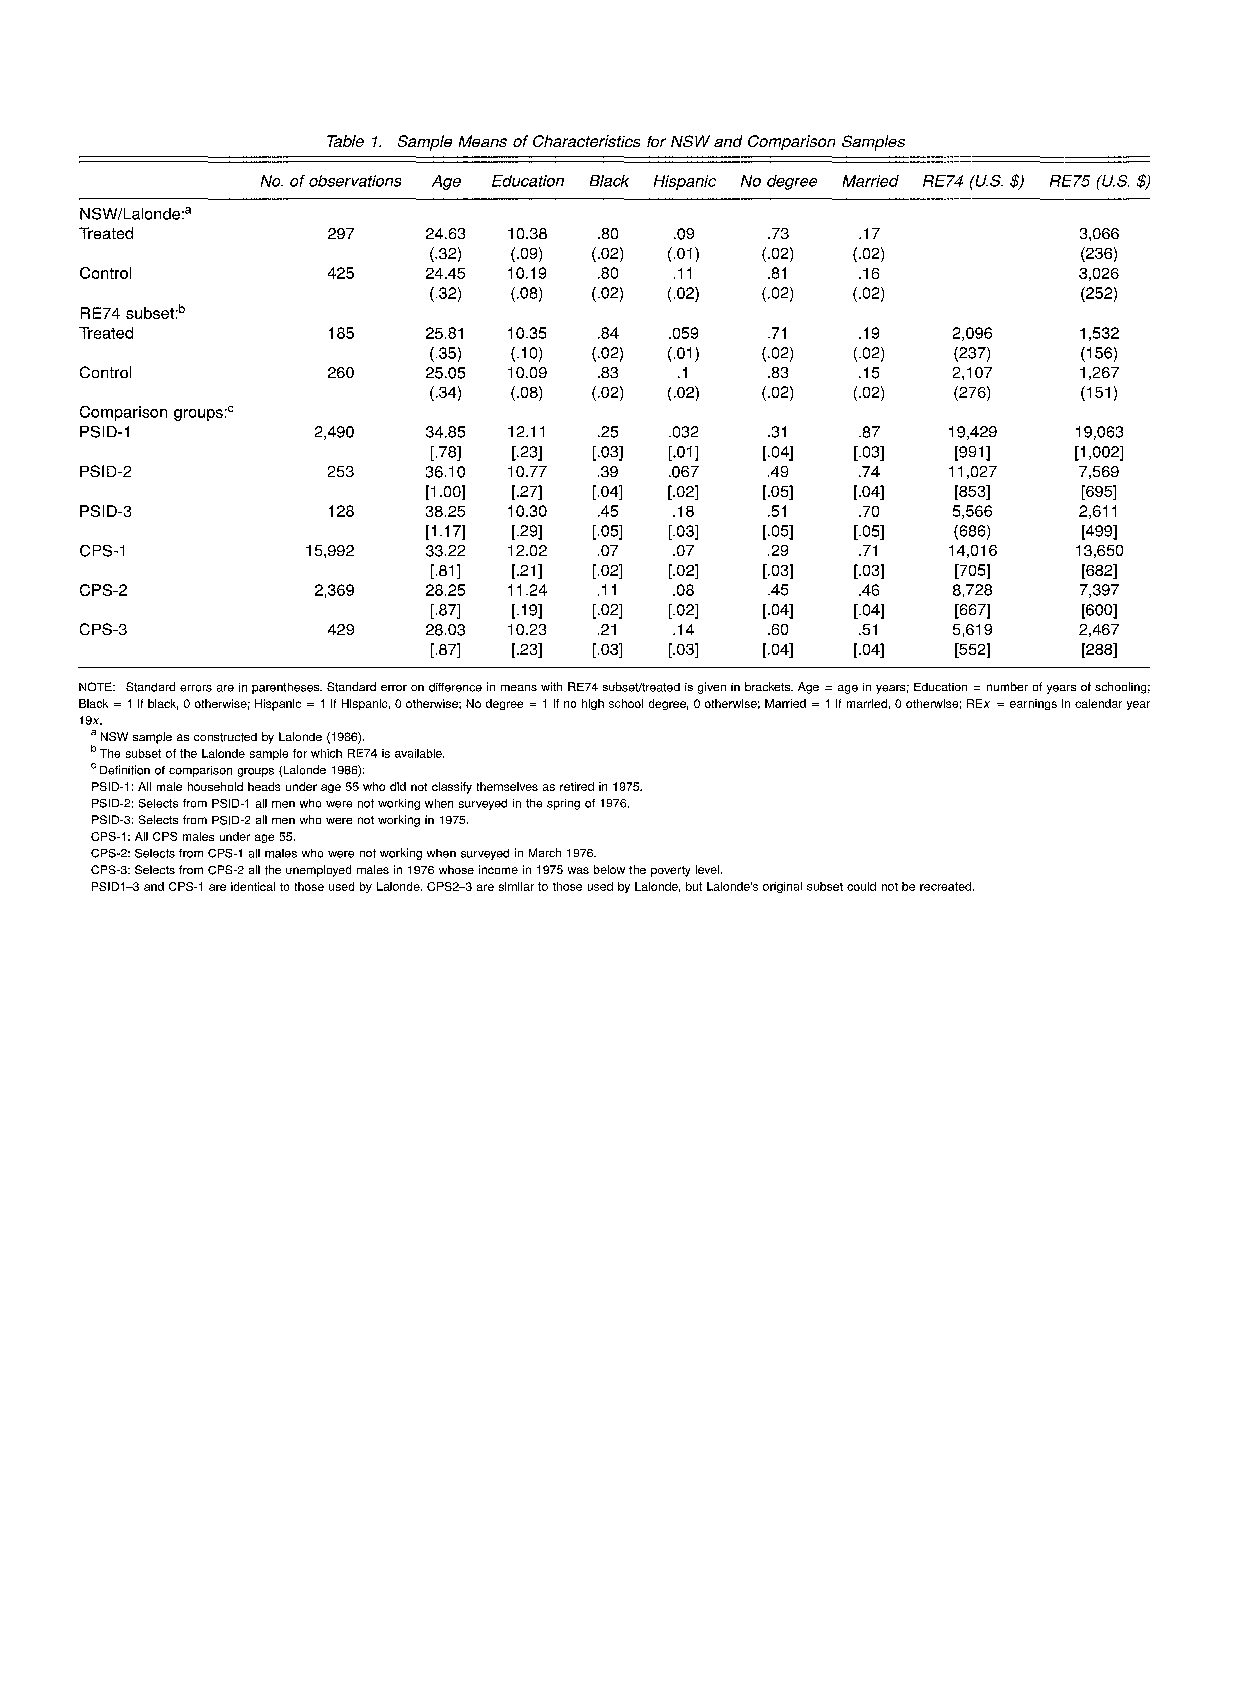
\includegraphics[scale=0.5]{./lecture_includes/dw_1.pdf}
\end{figure}

\end{frame}

\imageframe{./lecture_includes/dw_2.pdf}

\begin{frame}{Covariate imbalance}
	

	\begin{itemize}
	\item Conditional on the propensity score, the covariates are independent of the treatment, suggesting that the distribution of covariate values should be the same for both treatment and control groups
	\item This can be checked as we have data on all three once we've estimated the propensity score
	\item DW note that the two samples have \emph{severe} imbalance on \emph{observables} -- a huge number of non-experimental controls have propensity scores almost exactly equal to 0
	\item Their analysis will ``trim'' (which will ultimately have implications for interpretation)
	\end{itemize}

\end{frame}



\imageframe{./lecture_includes/dw_3.pdf}
\imageframe{./lecture_includes/dw_4.pdf}
\imageframe{./lecture_includes/dw_5.pdf}
\imageframe{./lecture_includes/dw_6.pdf}





\clearpage
\newpage

\begin{frame}{Replies by econometricians to DW}

\begin{itemize}
\item Heckman, Smith and Todd concluded from their own work that in order for matching estimators to have low bias, you need the following:
	\begin{enumerate}
	\item A rich set of variables related to program participation and predictive of $Y^0$ labor market outcomes, 
	\item Nonexperimental comparison group be drawn from the same local labor markets as the participants and 
	\item Dependent variable (e.g., earnings) be measured in the same way for participants and nonparticipants
	\end{enumerate}
\item All three of these conditions fail to hold in DW (1999, 2002) according to Smith and Todd (2005)
\item DW also note the importance of conditioning on pre-treatment lagged outcomes (e.g., real earnings in $t-1$, $t-2$, etc.) as well as \emph{trimming}
\end{itemize}

\end{frame}


\begin{frame}{Smith and Todd, diff-in-diff, doubly robust}

\begin{itemize}
\item Difference-in-differences with propensity scores tended to work well in Smith and Todd (2005) though the effect sizes are much larger
\item In my Causal Inference II workshop, we use Sant'anna And Zhao's double robust DiD and get nearly the exact same parameter estimate as the experimental finding

\end{itemize}

\end{frame}


\subsection{Coarsened exact matching}



\begin{frame}{Coarsened exact matching}
	
\begin{itemize}
\item There are two kinds of matching as we've said
	\begin{enumerate}
	\item \emph{Exact matching} matches a treated unit to all of the control units with the same covariate value. Sometimes this is impossible (e.g., continuous covariate). 
	\item \emph{Approximate matching} specifies a metric to find control units that are close to the treated unit. Requires a distance metric, such as Euclidean, Mahalanobis, or the propensity score.  All of which can be implemented in Stata's \texttt{teffects}.
	\end{enumerate}
\item 	Iacus, King and Porro (2011) propose another version of matching they call coarsened exact matching (CEM). Some big picture ideas
\end{itemize}
\end{frame}

\begin{frame}{Checking imbalance}

\begin{itemize}
\item Iacus, King and Porro (2008) say that in practice approximate matching requires setting the matching solution beforehand, then checking for imbalance after.  
\item Start over, repeat, until the user is exhausted by checking for imbalance.
\end{itemize}

\end{frame}

\begin{frame}{CEM Algorithm}
	
\begin{enumerate}
\item Begin with covariates $X$. Make a copy called $X*$
\item Coarsen $X*$ according to user-defined cutpoints or CEM's automatic binning algorithm
	\begin{itemize}
	\item Schooling $\rightarrow$ less than high school, high school, some college, college, post college
	\end{itemize}
\item Create one stratum per unique observation of $X*$ and place each observation in a stratum
\item Assign these strata to the original data, $X$, and drop any observation whose stratum doesn't contain at least one treated and control unit
\end{enumerate}

You then add weights for stratum size and analyze without matching.

\end{frame}

\begin{frame}{Tradeoffs}
	
	\begin{itemize}
	\item Larger bins mean more coarsening.  This results in fewer strata.  
	\item Fewer strata result in more diverse observations within the same strata and thus higher imbalance
	\item CEM prunes both treatment and control group units, which changes the parameter of interest.  Be transparent about this as you're not estimating the ATE or the ATT when you start pruning
	\end{itemize}
	
\end{frame}

\begin{frame}{Benefits}
	
	\begin{itemize}
	\item The key benefit of CEM is that it is in a class of matching methods called \emph{monotonic imbalance bounding}
	\item MIB methods bound the maximum imbalance in some feature of the empirical distributions by an ex ante decision by the user
	\item In CEM, this ex ante choice is the coarsening decision
	\item By choosing the coarsening beforehand, users can control the amount of imbalance in the matching solution
	\item It's also wicked fast.
	\end{itemize}
\end{frame}


\begin{frame}{Imbalance}
	
	\begin{itemize}
	\item There are several ways of measuring imbalance, but here we focus on the $\mathcal{L}_1(f,g)$ measure which is$$\mathcal{L}_1(f,g) = \frac{1}{2} \sum_{l_1 \dots l_k} | f_{l_1 \dots l_k} - g_{l_1 \dots l_k} |$$where the $f$ and $g$ record the relative frequencies for the treatment and control group units.
	\item Perfect global imbalance is indicated by $\mathcal{L}_1=0$.  Larger values indicate larger imbalance between the groups, with a maximum of $\mathcal{L}_1=1$. 
	\end{itemize}
\end{frame}

\begin{frame}{Stata}
	
	\begin{itemize}
	\item Download $\texttt{cem}$ from Stata:  \texttt{ssc install cem, replace}
	\item You will automatically compute the global imbalance measure, as well as several unidimensional measures of imbalance, when using $\texttt{cem}$
	\item I got a $\mathcal{L}_1=0.55$.  What does it mean?
		\begin{itemize}
		\item By itself, it's meaningless.  It's a reference point between matching solutions.
		\item Once we have a matching solution, we will compare its $\mathcal{L}_1$ to 0.55 and gauge the increase in balance due to the matching solution from that difference.
		\item Thus $\mathcal{L}_1$ works for imbalance as $R^2$ works for model fit: the absolute values mean less than comparisons between matching solutions.
		\end{itemize}
	\end{itemize}
	
\end{frame}

\begin{frame}{More Stata}
	
	\begin{itemize}
	\item Because $\texttt{cem}$ bounds the imbalance ex ante, the most important information in the Stata output is the number of observations matched.
	\item You can also choose the coarsening as opposed to relying on the algorithm's automated binning.  
	\item Once you have estimated the strata, you regress the outcome onto the treatment and then weight the regression by $\texttt{cem_weights}$.  For instance, $$\texttt{regress re78 treat [iweight=cem\_weight]}$$
	\item For more on this, see Blackwell, et al. Stata journal article from 2009.  
	\end{itemize}
\end{frame}




\section{Concluding remarks}

\begin{frame}{Comments}

\begin{itemize}

\item Selection on observables are important and when running regressions with controls, you are in fact doing it
\item Conditional independence requires that you \emph{know} and \emph{include} all confounders to adjust comparisons when estimating treatment effects
\item Without a prior behavioral model guiding you, it's very hard to defend conditional independence (borderline disingenuous) 
\item If you are unwilling to use DAGs, you may want to ask yourself why you are comfortable running regressions with covariates?

\end{itemize}

\end{frame}

\begin{frame}{When not to use selection on observables}

\begin{itemize}
\item Conditions for selection on observables are strong and subtle
\begin{enumerate}
		\item $(Y^1,Y^0) \independent{D} | X$ (conditional independence)
		\item $0<Pr(D=1|X)<1$ with probability one (common support)
\end{enumerate}
\item What exactly does the first thing mean?
		\begin{itemize}
		\item Easy to explain part: all the confounders are known and in your dataset
		\item Not as easy to explain part: once you condition on those things, your customers or people were behaving \emph{randomly}
		\end{itemize}
\item A lot of matching and weighting focused on biases created by dimensionality problems, but fixing those does not fix first point (and King and Nielsen are only focused on second)
\end{itemize}

\end{frame}  

\begin{frame}{Rationality issues}

\begin{itemize}
\item Roy models basically suggest people usually do things because it benefits them -- called ``selection on gains''
	\begin{itemize}
	\item If I do something, it's because $Y^1-Y^0>0$
	\item If I don't, it's because $Y^1-Y^0<0$
	\end{itemize}
\item We tend to think of this as nearly identical to rationality or intentional behavior, and when we use selection on observables methods we assume that that rationality could be absorbed by observables
\item Very mysterious idea and Smith and Sweetman (2015) suggest some kinds of behavior may not \emph{ever} satisfy this condition
\end{itemize}

\end{frame}



\begin{frame}{Comments}

\begin{itemize}

\item One diagnostic feature of the matching, weighting and imputation methods over OLS is the steps involved to evaluate common support
\item Unnecessary though -- you can incorporate the propensity score into regressions as weights
\item Nevertheless as we saw with DW, simply trimming can address some of the problems with overlap and propensity score makes this easier by collapsing $K$ strata into a single scalar
\item Histograms help to diagnoses these problems

\end{itemize}

\end{frame}

\begin{frame}{Comments}

\begin{itemize}

\item Don't hyper-critical or naive -- CIA may or may not hold in your data.  You can have too strong of priors in either direction
\item All that selection on observables does is create ``look-a-likes'' on \emph{observables}, but if you left out a critical confounder, you've not fixed anything
\item Adjusting for covariates may still be valuable even if you are worried about confounders as it can at least you know the differences are due to these known confounders

\end{itemize}

\end{frame}



\begin{frame}{Brief conclusion}

\begin{quote}
 ``All models are wrong but some are useful'' -- George Box
 \end{quote}
 
 \begin{itemize}
 \item Keep in mind -- you need to know your data, the area you're in, the people you're studying. 
 \item Data, credentials and classwork are not a substitute for common sense and thoughtfulness. 
 \item Sometimes CIA isn't insane and sometimes it may be and there is no rule I can give you

\end{itemize}

\end{frame}

\end{document}
